\chapter{Interference}
% Lesson Six: Interference

In this chapter, we will talk about one of the most fundamental phenomena concerning waves: interference. We will start by considering interference with normal single frequency waves when they superpose. Then we will move to interference of single photons, and we will conclude with interference of qubits.

\section{Constructive and destructive interference}


% Step One: Constructive and Destructive Interference

Let's consider that we have a single frequency wave propagating in time. How do we write down a mathematical expression that describes the propagation of such a wave? Well, we do it as follows:

\if0
\begin{equation}
\begin{array}{ll}
E_{1}=E_{01} \sin \left(\omega t+\alpha_{1}\right), & \alpha_{1}=-\left(k x+\phi_{1}\right) \\
E_{2}=E_{02} \sin \left(\omega t+\alpha_{2}\right), & \alpha_{2}=-\left(k x+\phi_{2}\right)
\end{array}
\end{equation}


\begin{equation}
E = E_0 sin(\omega t - \alpha)
\end{equation}
\fi

\begin{equation}
E=E_0 \sin [\omega t-(k x+\phi)].
\end{equation}
We denote the wave with $E$, and it's some constant $E_0$ ("E naught") times the sine of the following argument, where $E_0$ designates the \emph{amplitude} of oscillations, which means how much the wave is displaced from its rest state. The symbol $\omega$ (small omega) is the \emph{angular frequency}, which determines how quickly the wave is propagating in time. Time is denoted by $t$. $k$ is the \emph{wave number}. It's related to how fast the wave is propagating as well, and in three dimensions, it also gives you the direction of propagation. However, we are only considering propagation in one dimension, therefore it's just a scalar (a number). Finally, $\phi$ (small phi) is called the initial phase.

$\omega$, the angular frequency, is related to the period of oscillations as follows,
\begin{equation}
\omega=\frac{2 \pi}{T} \quad k=\frac{2 \pi}{\lambda}
\end{equation}
where $k$, the wave number, is related to $\lambda$ (lower case lambda), the wavelength of the oscillations, as shown. Let's have a look at some examples.

Let's freeze the wave at time $t=0$, and for convenience we also set $\phi = 0$, and only vary $k$. The blue wave in Fig.~\ref{fig:two-waves} is for $k=1$, whereas the orange one is for $k=0.5$, and the distance between the two dots at the top of the blue wave and bottom of the orange wave represents the wavelength of the wave. As we said, the wave number $k$ is related to the wavelength. The larger the wave number, the shorter the wavelength, so we see for $k=1$, the wavelength is shorter than for $k=0.5$.

Now, let's consider what happens when we fix the wave number but we vary the initial phase, as in Fig.~\ref{fig:phase-diff-waves}. The only thing that happens is that we shift the wave along the X-axis. We are just translating the wave a little bit by this angle, by this initial phase $\phi$. In this case, we have shifted the two waves by an initial phase of $\pi/2$, but this doesn't really affect how fast the wave is propagating, nor does it affect its wavelength.

So finally, let's add time dependence into the picture, as in Figs.~\ref{fig:two-waves} and \ref{fig:propagating-waves}. We set $k=1$, and we also set the initial phase $\phi=0$, and now the waves are actually propagating in time. For the first wave represented by the blue, we have $\omega=0.1$, whereas for the second wave we have $\omega=0.2$. Remember, we said that $\omega$ determines how fast the wave is propagating in time, and we can clearly see that the orange wave is faster than the blue wave.

Now, let's consider two waves that are actually interacting together and creating a new, third wave. How do we describe this new disturbance? So let's say that we have two waves, $E_1$ and $E_2$, each with different amplitude, same frequency, and we grouped the spatial variation into these factors $\alpha$: $\alpha_1$ and $\alpha_2$.

\begin{equation}
\begin{array}{ll}
E_1=E_{01} \sin \left(\omega t+\alpha_1\right), & \alpha_1=-\left(k x+\phi_1\right) \\
E_2=E_{02} \sin \left(\omega t+\alpha_2\right), & \alpha_2=-\left(k x+\phi_2\right)
\end{array}
\label{eq:superposition}
\end{equation}

This new wave that $E_1$ and $E_2$ produce is actually relatively simple, you just add them together
\begin{equation}
E=E_1+E_2.
\end{equation}
This is known as the \emph{principle of superposition}, and the idea is that we are looking for a description of the new resultant wave of the form
%, where now we have to find out what is this new amplitude $E_0$ in terms of the composite waves, and also we want to find out this new factor of $\alpha$.
\begin{equation}
E=E_0 \sin (\omega t-\alpha),
\end{equation}
so we need to determine the values for $E_0$ and $\alpha$. Using the trigonometric identity $\sin (a + b)=\sin a \cos b +\cos a \sin b$, we can rewrite Eq.~\ref{eq:superposition} as
\begin{equation}
\begin{aligned}
E &=E_{01}\left(\sin \omega t \cos \alpha_{1}+\cos \omega t \sin \alpha_{1}\right) \\
&+E_{02}\left(\sin \omega t \cos \alpha_{2}+\cos \omega t \sin \alpha_{2}\right)
\end{aligned}
\end{equation}
%, so let's see how we can do that. We just add the two waves together, and we begin by expanding these sines. The first wave can be written as this (see pointer)- we have the initial amplitude of the first wave, E zero one, and then we have sine omega t times cos alpha one, plus cos omega t times sine alpha one, and similarly for the second wave. 
We add them together, then group the time dependent terms. 
%So we see that these two terms (blue box), they both vary in time as sine omega t, whereas these two terms (red box) vary as cos omega t. So let's group them together and 
We get the following expression: 
%we have some spatial variation here, times sine omega t, and another spatial variation here, times cos omega t. And what we can do now is 

\begin{equation}
\begin{aligned}
E &=\left(E_{01} \cos \alpha_{1}+E_{02} \cos \alpha_{2}\right) \sin \omega t \\
&+\left(E_{01} \sin \alpha_{1}+E_{02} \sin \alpha_{2}\right) \cos \omega t
\end{aligned}
\end{equation}
We can define
%E naught cos alpha as the whole first expression to the left of $\sin\omega t$, and E naught sine alpha as the second expression.

\begin{equation}
\begin{aligned}
&E_{0} \cos \alpha=E_{01} \cos \alpha_{1}+E_{02} \cos \alpha_{2} \\
&E_{0} \sin \alpha=E_{01} \sin \alpha_{1}+E_{02} \sin \alpha_{2}
\end{aligned}
\end{equation}

And now with a little bit of algebra, we arrive at the following expression:

\begin{equation}
\begin{aligned}
E_{0}^{2} &=E_{01}^{2}+E_{02}^{2}+2 E_{01} E_{02} \cos \left(\alpha_{2}-\alpha_{1}\right)
\end{aligned}
\label{eq:superposition-simplified}
\end{equation}
We can find our overall value for $\alpha$ using the expression
\begin{equation}
\begin{aligned}
\tan \alpha &=\frac{E_{01} \sin \alpha_{1}+E_{02} \sin \alpha_{2}}{E_{01} \cos \alpha_{1}+E_{02} \cos \alpha_{2}}.
\end{aligned}
\label{eq:superposition-alpha}
\end{equation}

% so if we square this first expression (follow pointer) and add it to the square of the second expression, cos squared alpha plus sine squared alpha is equal to one (that's a very important trigonometric identity), so on this side (blue box LHS) we get E naught squared, and then we just have the squares which we have expanded over here (RHS) and simplified with some trigonometric identities. Also, if we take this orange expression, the second expression over here, and we divide by this blue expression over here, we can get an expression for tangent of alpha given as this following ratio. And this is our new wave.

We started with two waves with the same frequency, which means that the resultant disturbance also travels at the same frequency, which makes sense, but this new wave has different amplitude and also different phase. Before we look at an example, let's look at the amplitude of the superposition. The amplitude squared is equal to the sum of the squares of the component amplitudes, which makes sense. But then, there is the extra term on the end of Eq.~\ref{eq:superposition-simplified}, and this extra term is very important. It's called the \emph{interference term}. You can see that it actually oscillates as a result of the difference $\delta = \alpha_2 - \alpha_1$. This difference is called the "phase difference". The entire expression for $E_0^2$ is maximized when $\delta$ is either zero or multiples of $2\pi$, which we call \emph{constructive interference} because it's adding to the new resultant amplitude. On the other hand, if the phase difference is an odd integer multiple of $\pi$, e.g. $\pm\pi$ or $\pm 3\pi$, then what we get is \emph{destructive interference}.

Let's look at the example in Fig.~\ref{fig:decaying-superposition}. For convenience, we set the amplitudes of the two waves $E_1 = E_2 = 1$ and $\omega = 0.1$. The only thing that is different between them is their wave numbers $k$,
\begin{equation}
\begin{aligned}
&E_{1}=\sin (0.1 t-x) \\
&E_{2}=\sin (0.1 t-0.8 x) \\
&E=E_{1}+E_{2}.
\end{aligned}
\end{equation}
For the first wave $k=1$, for the second wave $k=0.8$. We add the two together and we get the following: with the blue and orange waves, we see the waves traveling independently, whereas the green wave is the superposition of these two waves, and you can see the interference at play. At the beginning, where $x$ is small, the waves travel in such a way that the crest of one wave seems to be on top of the crest of the other wave. Therefore, we get constructive interference. The waves are reinforcing each other, adding together producing something larger. Whereas, as the wave propagates into the region of larger $x$, they are propagating at different speed. They go out of phase, so the crest of one wave is meeting the trough of the other wave, so they are destructively interfering. They're cancelling each other out, and we can see that in the green wave, where the amplitude becomes very low, nearly zero. And that's how interference works.

\if0
\begin{equation}
E=E_{0} \sin [\omega t-(k x+\phi)]
\end{equation}
% k=1, k=0
$\phi = 0$ and $\phi = \frac{\pi}{2}$
\fi

\begin{figure}[H]
   \centering
    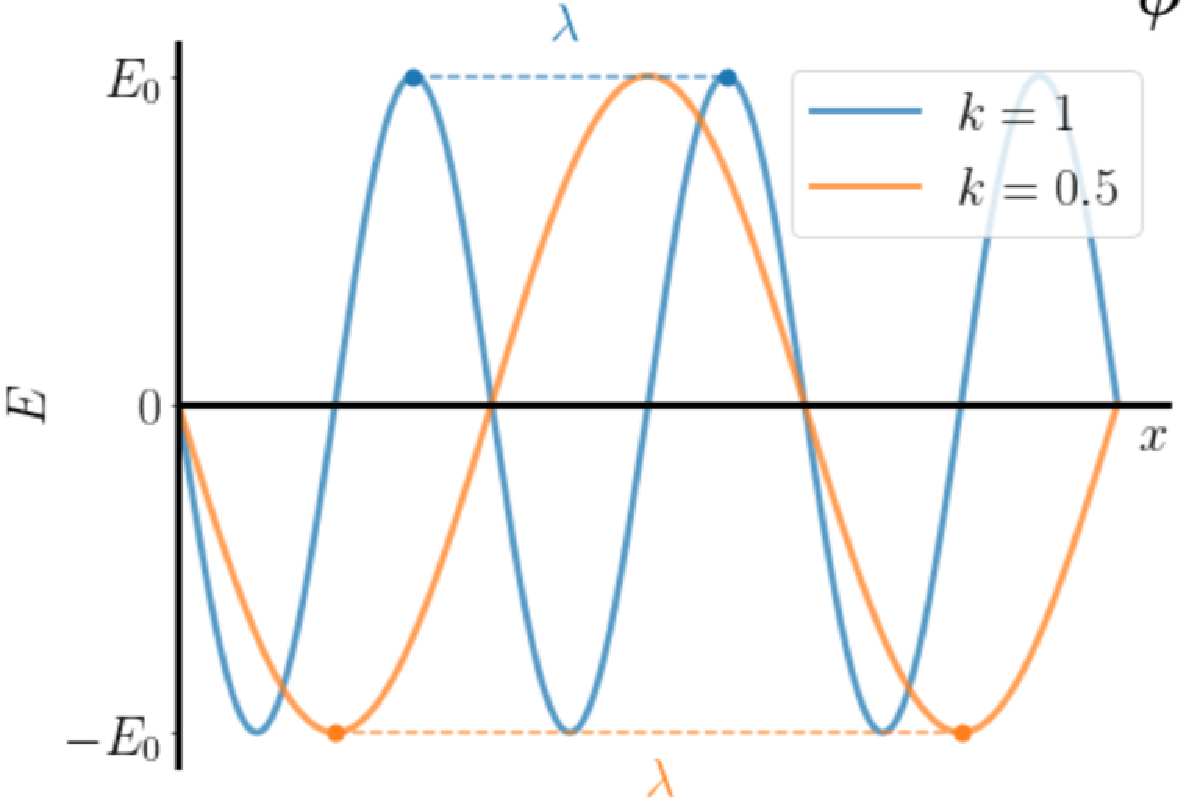
\includegraphics[width=0.8\textwidth]{lesson6/k.pdf}
        \caption{Two independent waves with $k=1, k=0.5$}    
    \label{fig:two-waves}
\end{figure}

% phi = 0, phi = pi/2
\begin{figure}[H]
   \centering
    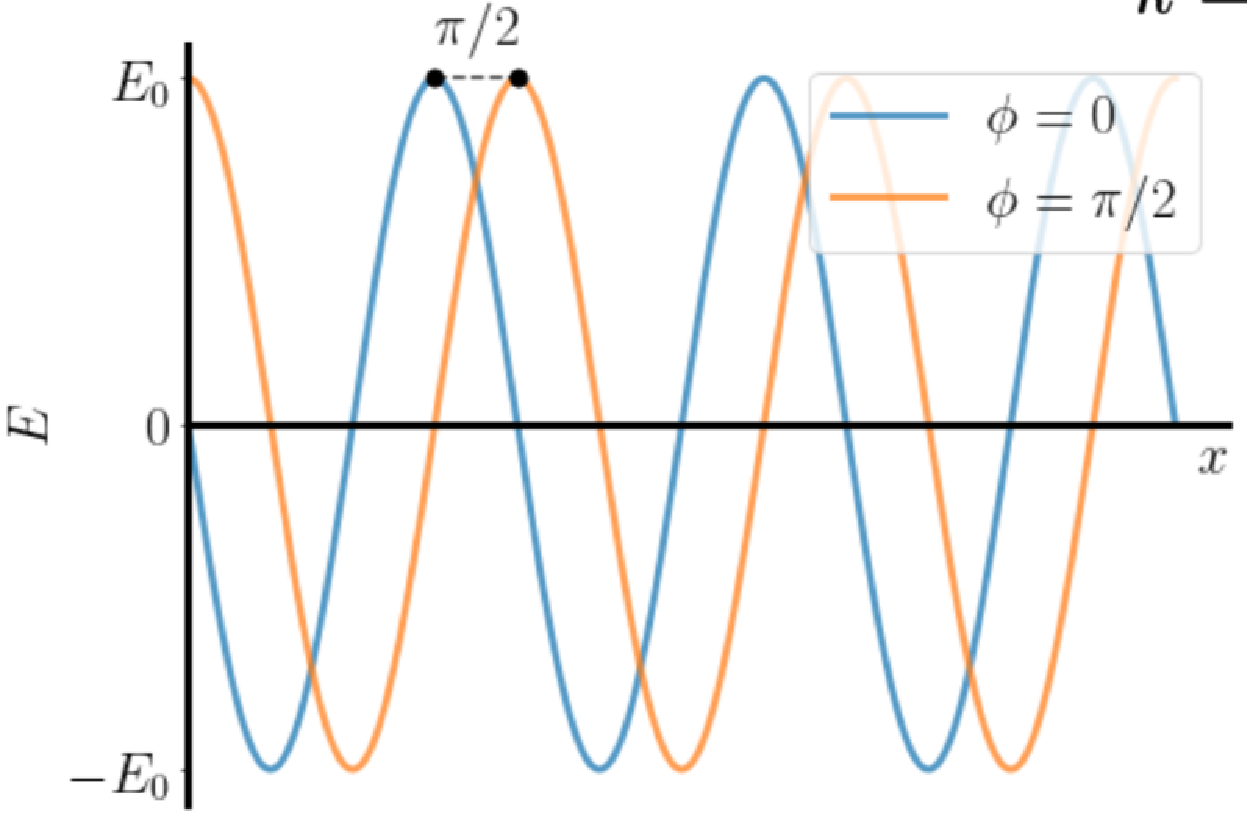
\includegraphics[width=0.8\textwidth]{lesson6/phi.pdf}
        \caption{Two waves with the same wavelength but different initial phase, $\phi = 0, \phi = \pi / 2$.}
    \label{fig:phase-diff-waves}
\end{figure}

% gif two waves [insert pic]
\begin{figure}[H]
   \centering
    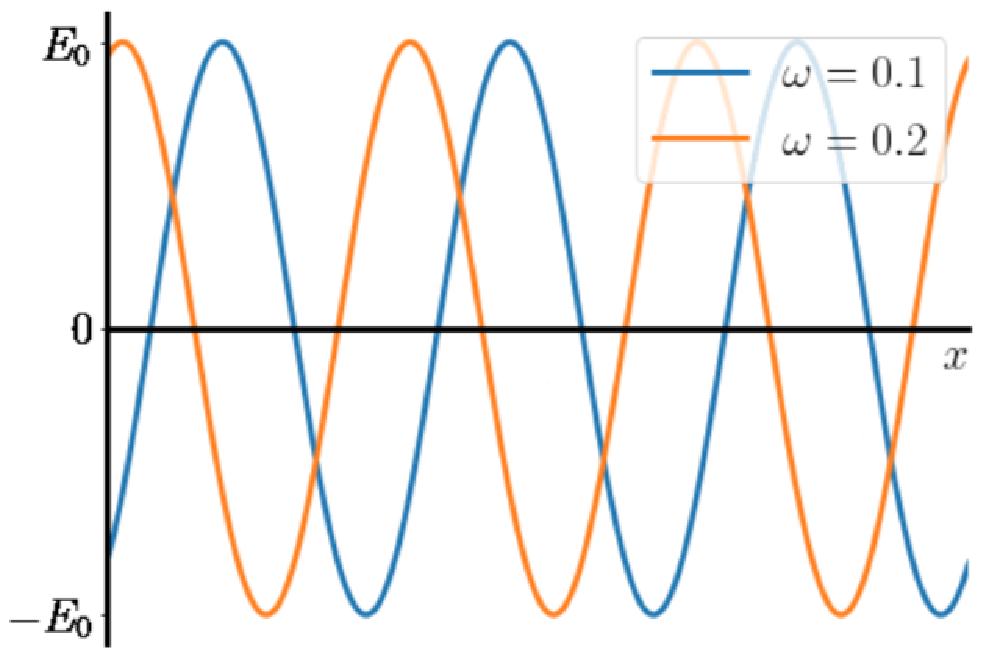
\includegraphics[width=0.8\textwidth]{lesson6/w.pdf}
        \caption{The same two waves as in the previous figure, after some time.  The orange wave propagates faster than the blue wave.}
    \label{fig:propagating-waves}    
\end{figure}

% superposition two waves
\begin{figure}[H]
   \centering
    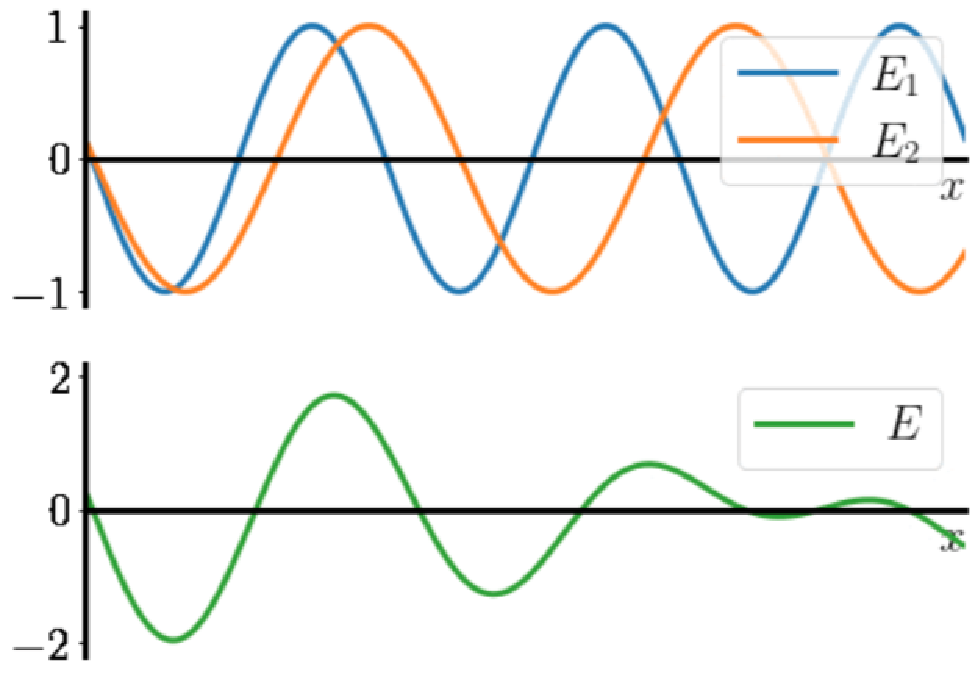
\includegraphics[width=0.8\textwidth]{lesson6/wave_superposition.pdf}    
        \caption{Waves in superposition. Notice the decay of the green wave as the two component waves move from in phase to out of phase.}
    \label{fig:decaying-superposition}    
\end{figure}

%%%%%%%%%%%%%%%%%%%%%%%%%%%%%%%%%%%%%%%%%%%%%%%%%%%%%%%%%%%%%%%%%%%%%%%%%%%%%%%%
\section{Phase and group velocities}
\label{sec:6-2_phase_group_velocity}
%%%%%%%%%%%%%%%%%%%%%%%%%%%%%%%%%%%%%%%%%%%%%%%%%%%%%%%%%%%%%%%%%%%%%%%%%%%%%%%%

In this section, we will investigate the speed at which a wave propagates.
We will begin by considering how the speed of propagation for waves of single frequency before moving onto more complicated waves resulting from interference of multiple waves.

First, let's consider a single wave of a single frequency propagating through space and ask the question: at what speed does this wave travel?
We saw in the previous section that we can write down such a wave as
\begin{equation}
    E = E_{0} \sin (\omega t-k x-\phi),
\end{equation}
where the phase at a particular point in time $t$ and space $x$ is $\theta(x,t)=\omega t-k x-\phi$.
Since the wave is described by a single frequency, the speed of propagation of the wave is given by the speed of point of constant phase.
How fast does this point of constant phase propagate?
To answer this question we just need to differentiate the expression for phase with respect to time and set it equal to zero,
\begin{equation}
    \frac{d\theta(x,t)}{d t} = \omega - k\underbrace{\frac{dx}{dt}}_{= v_p} = 0, \longrightarrow v_p = \frac{\omega}{k}.
    \label{eq:6-2_phase_velocity}
\end{equation}
We have defined a new quantity called the \textit{\textbf{phase velocity}} $v_p$.

\begin{figure}[t]
   \centering
    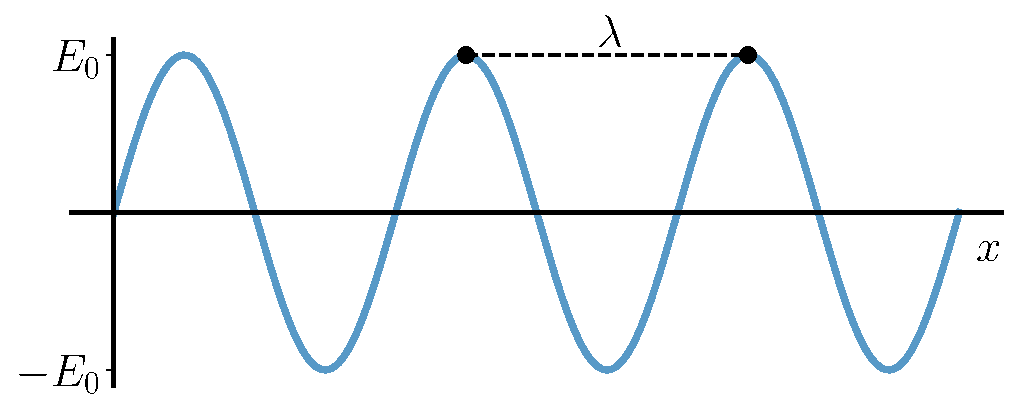
\includegraphics[width=0.8\textwidth]{lesson6/6-2_phase_velocity.pdf}    
        \caption[Phase velocity]{The black points represent points of same phase and are separated by the wavelength $\lambda$.}
        \label{fig:6-2_phase_velocity}
\end{figure}

We can check that the expression for phase velocity in Eq.~(\ref{eq:6-2_phase_velocity}) makes sense in the following way.
Consider two points on the wave with same phase as shown in Fig.~\ref{fig:6-2_phase_velocity}.
These points are separated by a distance of exactly one wavelength $\lambda$.
The time needed for the left black point to traverse this distance is one period $T$;
therefore, the speed at which the wave moves is given by the ratio $\lambda / T$.
The wavelength of the wave can be expressed in terms of the wave number, $\lambda = 2\pi / k$.
Similarly, the period can be written in terms of the frequency, $T = 2\pi / \omega$.
The speed of propagation can then be written as
\begin{equation}
    \frac{\frac{2\pi}{k}}{\frac{2\pi}{\omega}} = \frac{\omega}{k} = v_p,
\end{equation}
which is the phase velocity of Eq.~(\ref{eq:6-2_phase_velocity}).

% Let's look at an example. We have a wave propagating at angular frequency $0.1$ and the wave number is $1$,
% \begin{equation}
% E=\sin (0.1 t-x).
% \end{equation}
% And then, as you can see, I marked one black point here (follow pointer), this is a point of constant phase and it's propagating through space like that.

How is the speed of the wave affected when the wave itself is a superposition of multiple single-frequency waves?
Let's take two waves. This time, we allow their angular frequencies to be different, but for simplicity assume the two waves to have same amplitude $E_0$,
\begin{align}
    E_1 & = E_0 \sin \left(\omega_1 t-k_1 x\right) \\
    E_2 & = E_0 \sin \left(\omega_2 t-k_2 x\right).
\end{align}
The phase velocities of these waves are given according to Eq.~(\ref{eq:6-2_phase_velocity}),
\begin{equation}
    v_{p1} = \frac{\omega_1}{k_1}, \qquad v_{p2} = \frac{\omega_2}{k_2}.
\end{equation}
\begin{figure}[t]
   \centering
    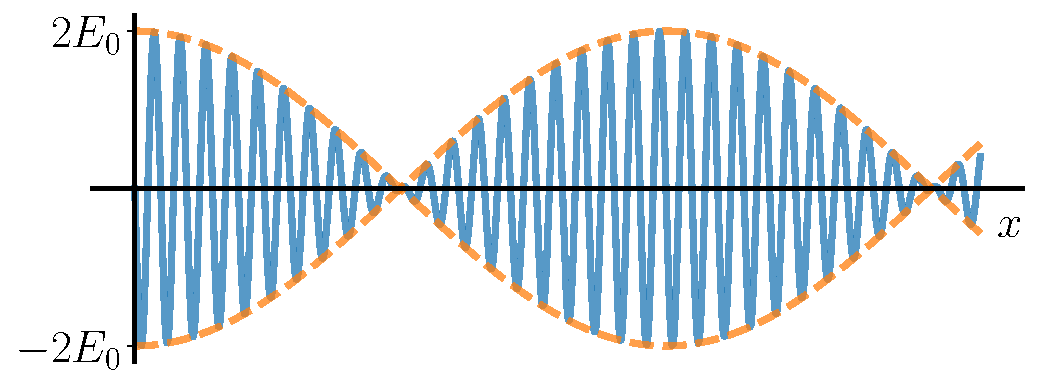
\includegraphics[width=0.8\textwidth]{lesson6/6-2_superpostion_velocity.pdf}    
        \caption[Group velocity]{Superposition of two sinusoidal waves. The fast oscillations are modulated by a slowly-varying envelope.}
        \label{fig:6-2_superposition}
\end{figure}
Let's compute an expression for the superposition,
\begin{align} 
    E & = E_{1} + E_{2} \nonumber\\
     & = E_{0}\left[\sin \left(\omega_{1} t-k_{1} x\right)+\sin \left(\omega_{2} t-k_{2} x\right)\right] \nonumber\\
    & = 2 E_{0} \underbrace{\sin \left( \frac{\omega_{1}+\omega_{2}}{2} t-\frac{k_{1}+k_{2}}{2} x \right)}_{\text{fast oscillations}} \underbrace{ \cos \left( \frac{\omega_{1}-\omega_{2}}{2} t-\frac{k_{1}-k_{2}}{2} x \right)}_{\text{slow oscillations}}.
\end{align}
We see that the superposition can be split into two terms.
The first captures the fast oscillations of the superposition at frequency $\omega_1+\omega_2$.
These fast oscillations are pictured in blue in Fig.~\ref{fig:6-2_superposition}.
Similar to the case of a single-frequency wave, we can ask the question at what speed a point of constant phase travels to obtain the \textit{\textbf{phase velocity}} for the superposition.
This information is contained in the fast-oscillation term of Eq.~(\ref{eq:6-2_phase_velocity}),
\begin{equation}
    v_p = \frac{\omega_1 + \omega_2}{k_1 + k_2}.
\end{equation}
These fast oscillations are modulated by a slowly-varying envelope as seen in by the oranged dashed line in Fig.~\ref{fig:6-2_superposition}.
This is captured by the second term in Eq.~(\ref{eq:6-2_phase_velocity}) and the frequency of these slow oscillations is $\omega_1-\omega_2$.
This term also gives rise to \textit{\textbf{group velocity}},
\begin{equation}
    v_g = \frac{\omega_1 - \omega_2}{k_1 - k_2}.
\end{equation}
It is the group velocity that tells us how fast the entire group travels.
The phase and group velocities of a superposition are, in general, different.
We can have scenarios where one is larger than the other but also where they are equal,
\begin{equation}
    v_p > v_g, \quad v_p = v_g, \quad v_p < v_g.
\end{equation}
Real wave packets and signals are rarely single-frequency waves but rather results of a superposition of a number of single-frequency components.
When we talk about the speed of such a wave, we usually refer to the group velocity.
It is also the group velocity that tells us how quickly a signal carries information.

% Let's illustrate it with an example. We consider two waves $E_1$ and $E_2$,
% \begin{equation}
% \begin{aligned}
% &E_{1}=\sin (0.1 t-2.0 x) \\
% &E_{2}=\sin (0.2 t-2.1 x).
% \end{aligned}
% \end{equation}
% They have different angular frequencies. $E_1$ has angular frequency $\omega_1 = 0.1$, whereas $E_2$ has angular frequency $\omega_2 = 0.2$. They have different wave numbers, as well. $E_1$ has $k_1 = 2.0$, and $E_2$ has $k_2=2.1$. So, let's plot this initially at time equals to zero, and as we said, we expect the shape of the superposition to to be composed of two waves. One is this fast oscillating blue line, and on top of that we have this slowly varying \emph{envelope}\index{envelope}. Again, this blue fast oscillating term is given by the sine term from previous slides, and this orange dashed line gives us the envelope which is proportional to the cosine. 
% Now let's get things moving, and in time again it propagates through space.

% So now, let's actually compute what the phase and group velocities are for our example. We just substitute into our expressions,
% \rdv{Are these expressions backwards?}
% \begin{equation}
% \begin{gathered}
% v_{p}=\frac{\omega_{1}+\omega_{2}}{k_{1}+k_{2}}=\frac{0.3}{4.1} \approx 0.07 \\
% %v_{g}=\frac{\omega_{1}-\omega_{2}}{k_{1}-k_{2}}=1 & 
% v_{g}=\frac{\omega_{1}-\omega_{2}}{k_{1}-k_{2}}=1 
% \begin{array}{l}
% \end{array} \\
% v_{g}>v_{p} \quad v_{g} \approx 14 v_{p}
% \end{gathered}
% \end{equation}
%so omega one plus omega two, we just add them together, so 0.1 plus 0.2 is 0.3. k1 plus k2, again we add them together, 2.0 plus 2.1 is 4.1. And this (v-p) is approximately 0.07 (zero point zero seven). For the group velocity, we do the same thing and we obtain that the group velocity is equal to one. 
% We can see that the group velocity in this case is larger than the phase velocity, and in fact it's about fourteen times larger.

% Let's go back to our propagating wave, so you can see what actually happens to the points on our wave. The black dot oscillating up and down represents our phase velocity. This black point is moving through space with the phase velocity, so you can see that it's moving up and down quite a lot, but actually it's not propagating through space very much, because it's in this example equal to 0.07, whereas this red square that occasionally you can see at the top, that goes zooming- it's sitting on the envelope over there and it goes to zooming through space. That point represents the group velocity. Well you can't actually see that it's fourteen times faster but mathematically that's true. And as we said in this case that we picked the phase velocity is smaller than the group velocity. But this is not always the case.

% Let's look at this following example: we kept the same angular frequencies for the two waves, but we changed the wave numbers. Now E1 has k equal to zero point one and E2 has k equal to zero point two. Let's see what that looks like. As you can see, now the group velocity and the phase velocity are the same. The black point and the red square move at the same velocity.

% \begin{equation}
% \begin{aligned}
% &E_{1}=\sin (0.1 t-0.1 x) \\
% &E_{2}=\sin (0.2 t-0.2 x)
% \end{aligned}
% \end{equation}

% So far, we have looked at cases when both velocities are in the same direction. Now, let's look at a very peculiar case.

% Again, we keep the angular frequencies fixed, but this time we change k1 to two point zero and k2 to one point five, and let's see what happens. You see that again, the black dot representing our phase velocity is moving in the positive x direction as was the case before, but on the other hand this red square is moving backwards, because the group velocity in this case is actually negative. So you can see that you can have a lot of fun with the group and phase velocities. there are many different scenarios depending on omega one and omega two and k1 and k2.


% \begin{equation}
% \begin{aligned}
% &E_{1}=\sin (0.1 t-2.0 x) \\
% &E_{2}=\sin (0.2 t-1.5 x)
% \end{aligned}
% \end{equation}

% So far, we have been looking at superposition of only two waves. What happens if we consider superposition of more than two waves?

\begin{figure}[t]
   \centering
    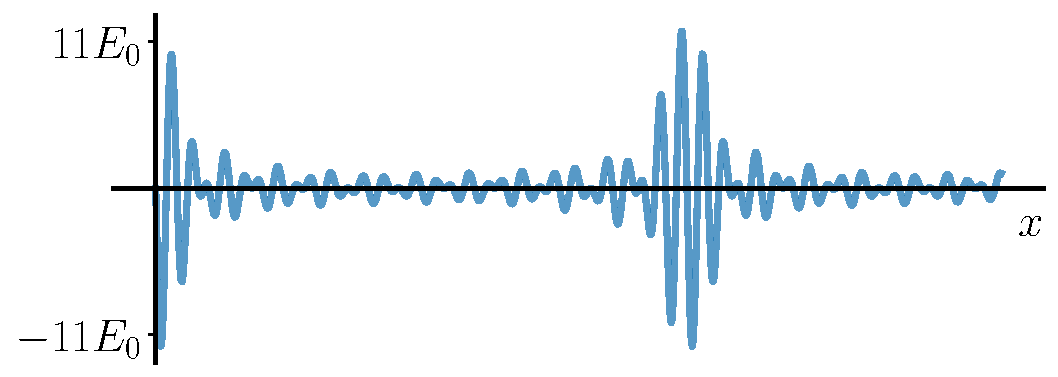
\includegraphics[width=0.8\textwidth]{lesson6/6-2_superpostion_many.pdf}    
        \caption[Pulse]{Superposition of multiple sinusoidal waves given in Eq.~(\ref{eq:6-2_pulse}).}
        \label{fig:6-2_pulse}
\end{figure}
We can consider the case where we interfere more than two single-frequency waves.
Let's say we have a superposition of the following form,
\begin{equation}
    E = E_0 [\sin(-2.0x) + \sin(-2.1x) + \ldots + \sin(-3.0x)].
    \label{eq:6-2_pulse}
\end{equation}
We have assumed that we are looking at the superposition frozen in time at $t=0$, hence the simple form.
The resultant superposition is pictured in Fig.~\ref{fig:6-2_pulse}.
Unlike before, we can observe long regions where destructive interference results in almost no disturbance.
Then the constructive interference kicks in and we observe a short \textit{\textbf{pulse}}.
It is these pulses that can be used to carry information at the group velocity of the superposition.



\section{Interference with single photons}
\label{sec:6-4_interference_single_photons}

% double_slit standard
\begin{figure}[H]
   \centering
    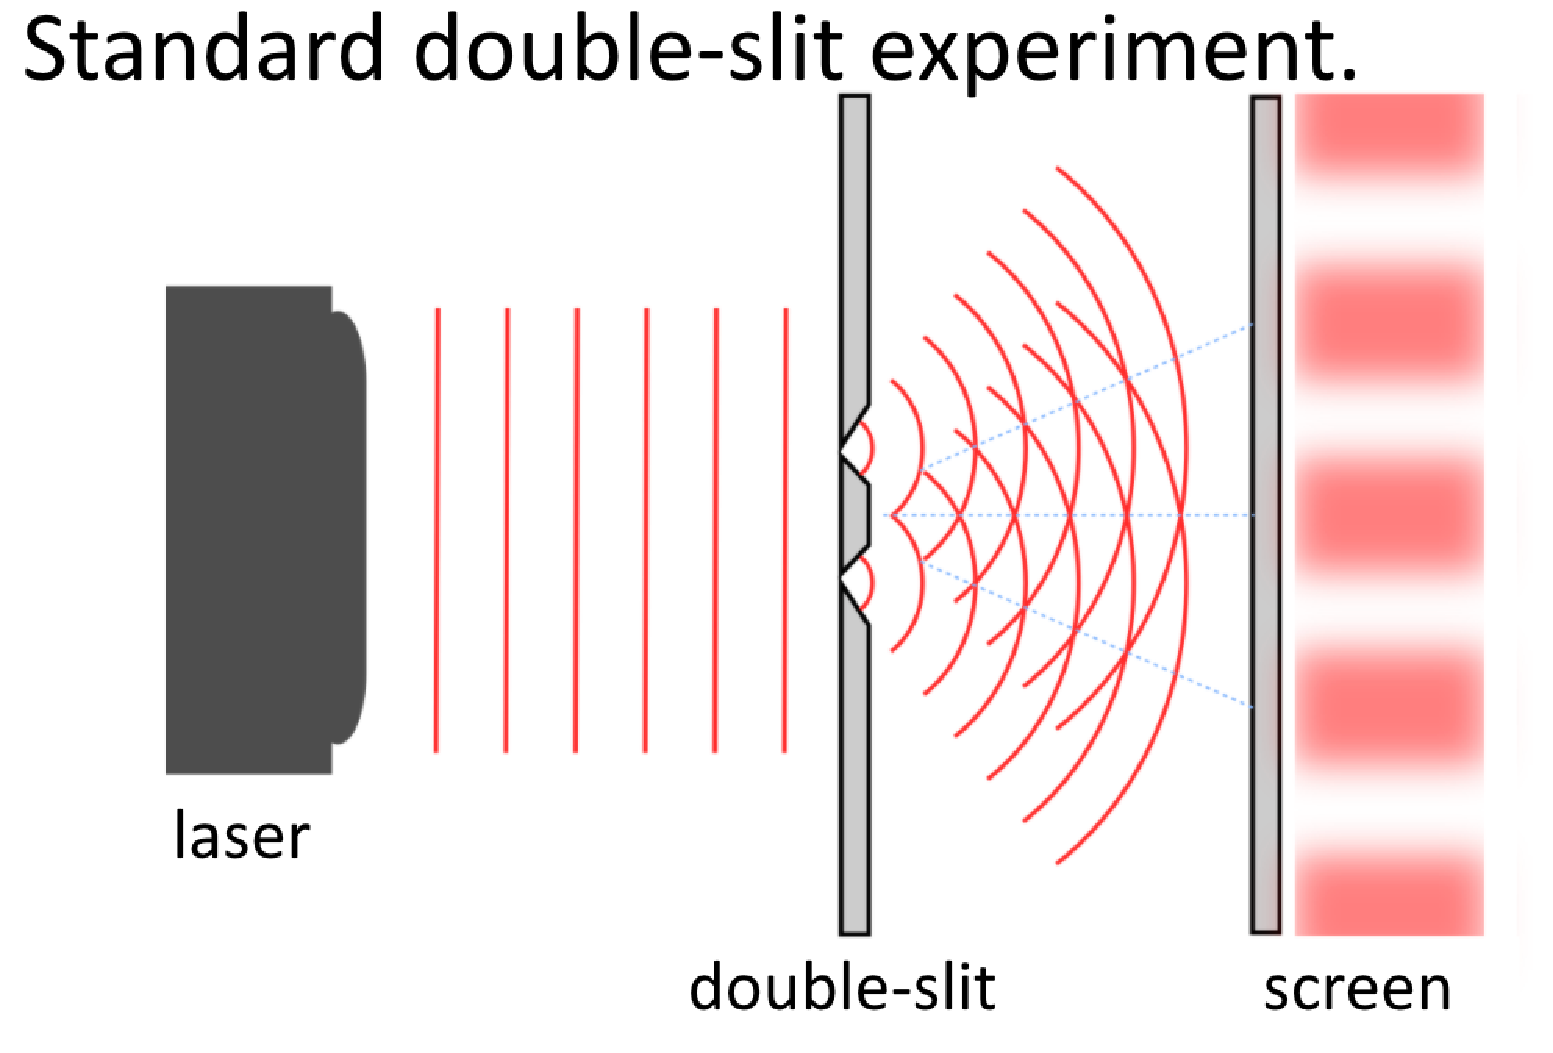
\includegraphics[width=0.8\textwidth]{lesson6/standard_double_slit.pdf}    
        \caption{The canonical two-slit experiment.}
    \label{fig:two-slit}
   
\end{figure}

I'm sure you have already seen the scenario of a double slit experiment with laser light in another of your physics classes, but let's review it again.

In this experiment we have a source of coherent light, canonically a laser. In Fig.~\ref{fig:two-slit}, the laser light is incident on a screen, where there are only two small slits where the light can go through, and then it propagates towards another screen where we detect a pattern. The pattern that we see looks something like this: we have fringes of bright light (pink in the figure), and then fringes where there is no light (blank, or white, in the figure). Why is that?  The pink lines represent the peaks of the electromagnetic waves. They are straight before coming to the screen, perpendicular to the direction of travel. After passing through the slits, they radiate out in a circular pattern.  Following the light blue lines, you can see that where the peaks from the two slits meet, the lines cross.  Those blue lines are where we get constructive interference, giving us the strong pink illumination on the screen. Halfway in between those blue lines, you can see that the wave from one slit is at its peak when the other is at its trough.  This will give us destructive interference.

% As you can see, as the light is propagating through here (follow pointer), these lines, they represent the peaks of the electromagnetic wave, whereas the space in between them represent the valleys, the troughs. So as the two waves go through these slits, they have a chance to interfere constructively or destructively. Where their peaks meet, the wave- the interference of the two waves reinforces their amplitude. On the other hand, if a peak meets a trough or a valley, then the amplitudes cancel, and here we can see these light blue lines, these are the lines along which we see constructive interference.

For example, consider the point right in the middle of the screen, as shown in Fig.~\ref{fig:two-slit-constructive}. The light coming from the top slit and light coming from the bottom slit travel the same distance. The path length of these two paths are equal, therefore there is no phase difference between the two waves coming from the top slit and the bottom slit, and we observe constructive interference. On the other hand, for the fringe above the middle, the path length for the top path is a little bit shorter than the bottom one. But the phase difference introduced for this case is exactly $2\pi$, which again, corresponds to constructive interference as we have seen in the previous section. Similarly for the top fringe in our figure, we have a phase difference of $4\pi$.
% constructive interference
\begin{figure}[H]
   \centering
    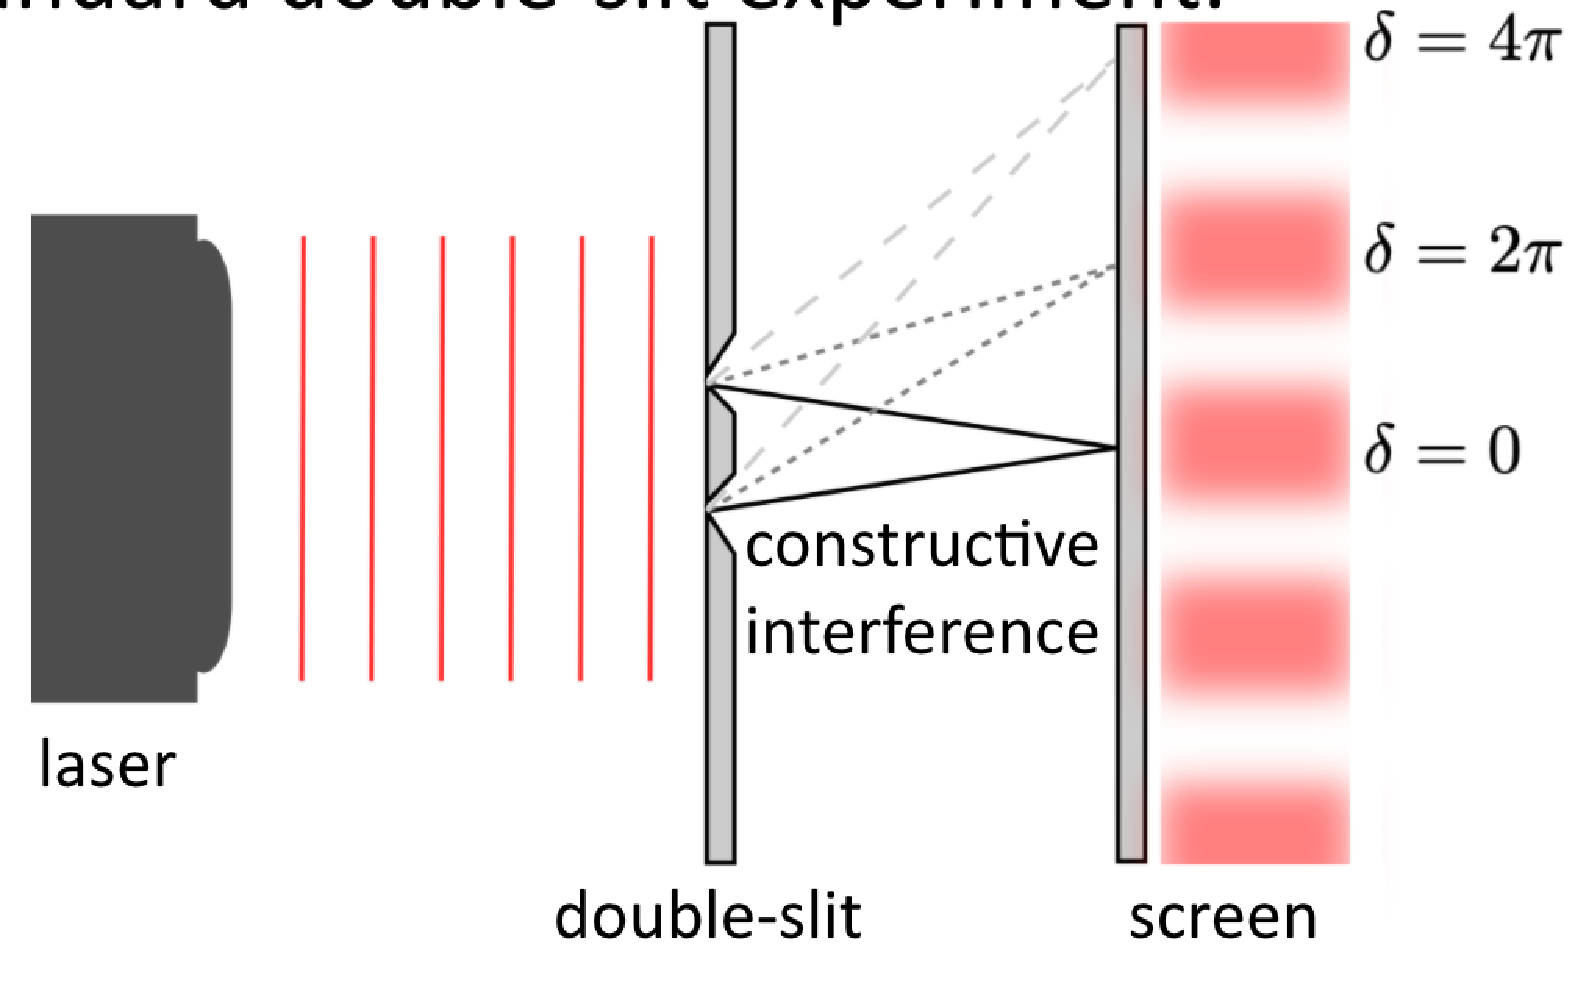
\includegraphics[width=0.8\textwidth]{lesson6/double_slit_constructive.pdf}    
        \caption{Constructive interference.}
    \label{fig:two-slit-constructive}    
\end{figure}

On the other hand, consider the paths shown in Fig.~\ref{fig:two-slit-destructive}. Along these paths, peaks meet the troughs, where the path differences are odd integer multiples of $\pi$. So for this first dark (blank white) region on the screen, we have the phase difference being $\pi$; for the second dark region on the screen, we have the phase difference being $3\pi$, and so on.

% destructive inteference
\begin{figure}[H]
   \centering
    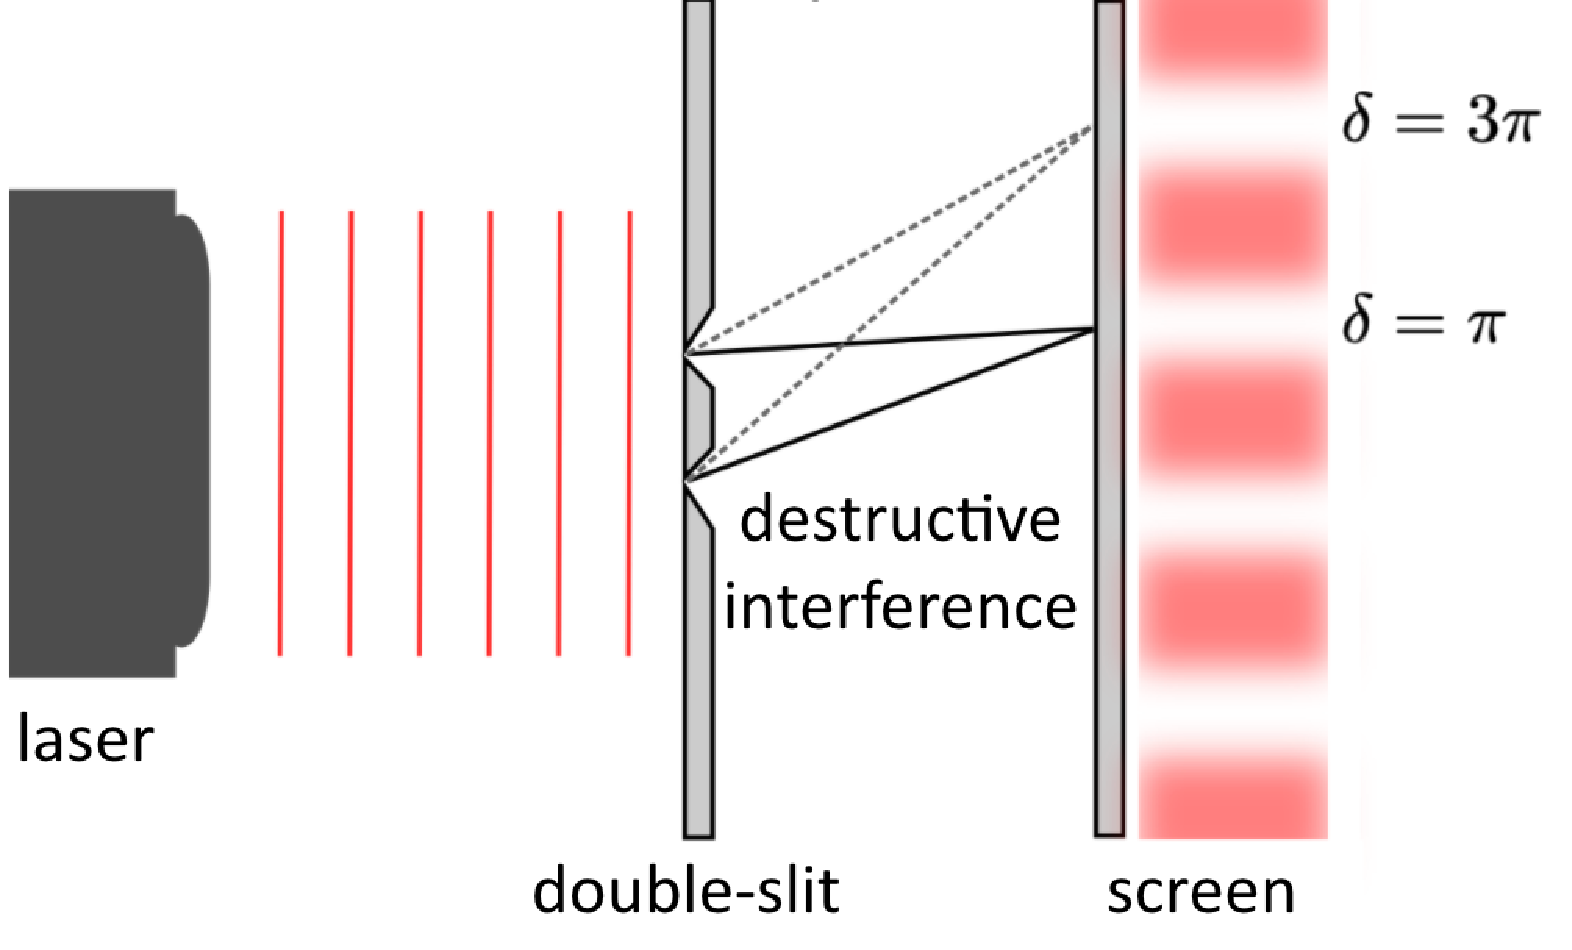
\includegraphics[width=0.8\textwidth]{lesson6/double_slit_destructive.pdf}
        \caption{Destructive interference.}
    \label{fig:two-slit-destructive}    
\end{figure}

Now, let's consider the scenario where we attenuate the laser light to such low levels that it's only firing single photons at a time, and furthermore, the level of attenuation is so high that we can be pretty sure that there's only one photon at a time between this screen where we place the double slits, and the screen where we are recording the pattern. So, what happens? Well, we know that the photons must go through one of these slits. So, let's try covering one of them. What do we expect? If we cover the bottom one, then definitely the photons have to go through the top slit in order to hit the screen, so we expect most of the photons hitting the screen will appear in the region that's the closest to the top slit, as in Fig.~\ref{fig:two-slit-lower-blocked}. On the other hand, if we block the top slit, as in Fig.~\ref{fig:two-slit-upper-blocked}, and the photons are allowed to pass through this bottom slit, then we expect most of the photons to be recorded on the lower portion of the screen. What happens if we open both of the slits, as in Fig.~\ref{fig:two-slit-single-photon-wrong}? They can go through the top, and they can go through the bottom, so we expect something like this: we expect that the two previous distributions are just added together. Is this really what we see? Well, let's find out. 

% attenuated laser
\begin{figure}[H]
   \centering
    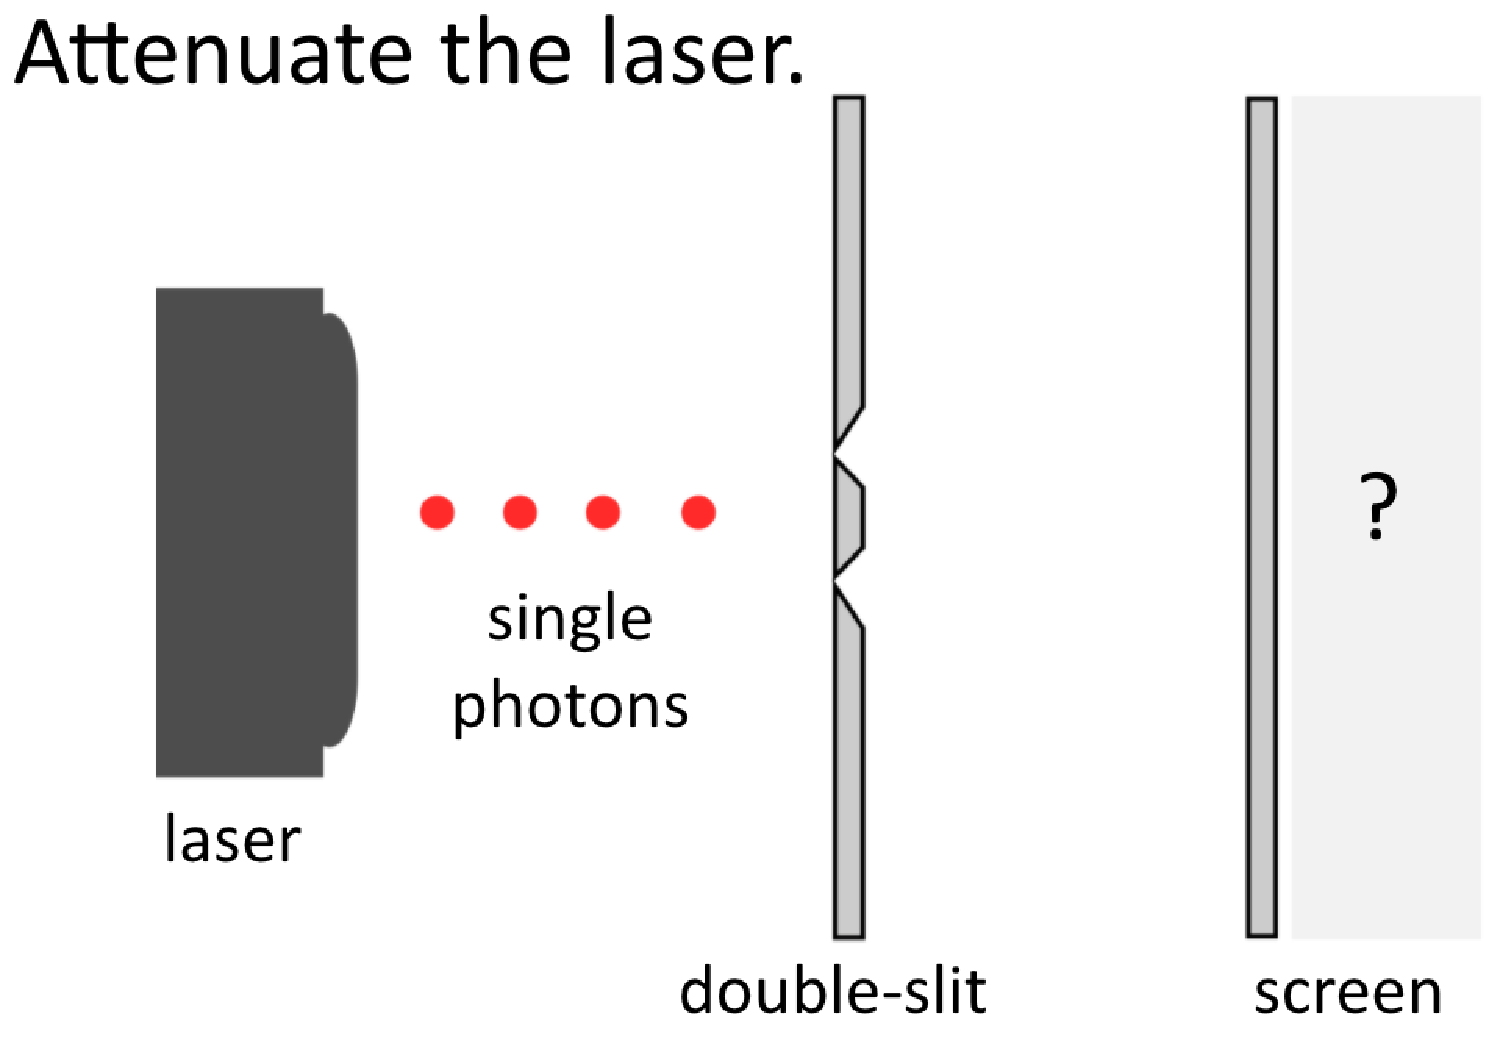
\includegraphics[width=0.8\textwidth]{lesson6/attenuate_laser.pdf}    
        \caption{Attenuated laser light.}
    \label{fig:two-slit-attenuated}
\end{figure}

% block bottom
\begin{figure}[H]
   \centering
    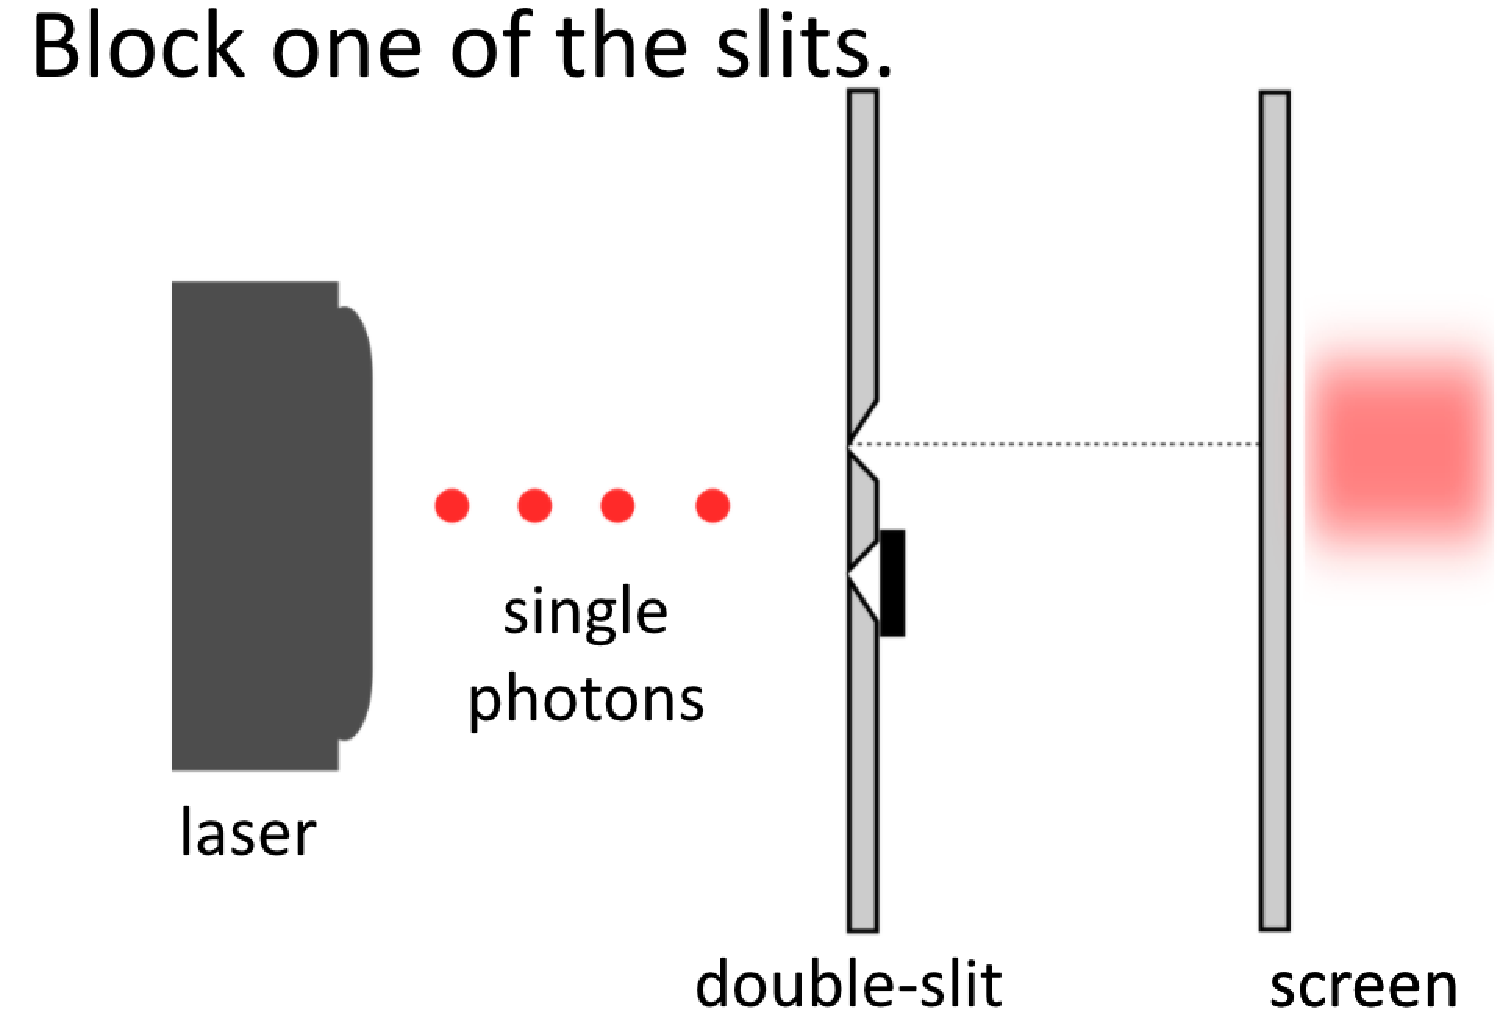
\includegraphics[width=0.8\textwidth]{lesson6/block_bottom.pdf}
    
        \caption{Pattern observed when the lower slit is blocked.}
    \label{fig:two-slit-lower-blocked}
    
\end{figure}

% block top
\begin{figure}[H]
   \centering
    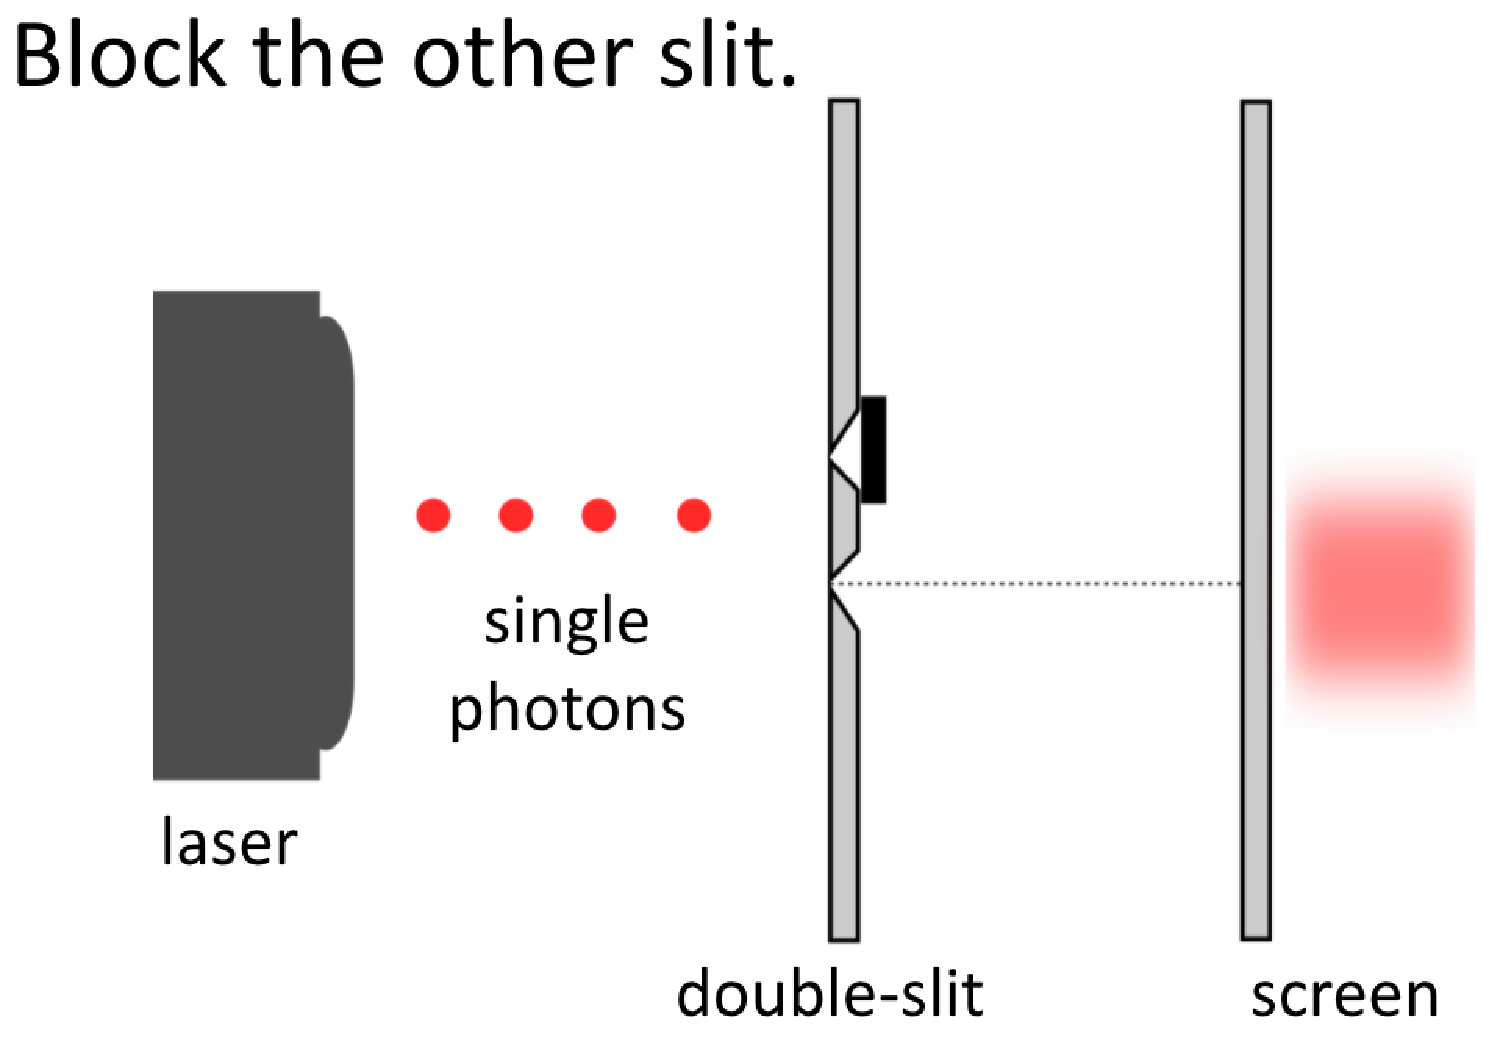
\includegraphics[width=0.8\textwidth]{lesson6/block_top.pdf}
    
        \caption{Pattern observed when the upper slit is blocked.}
    \label{fig:two-slit-upper-blocked}
    
\end{figure}


% block netiher expectation
\begin{figure}[H]
   \centering
    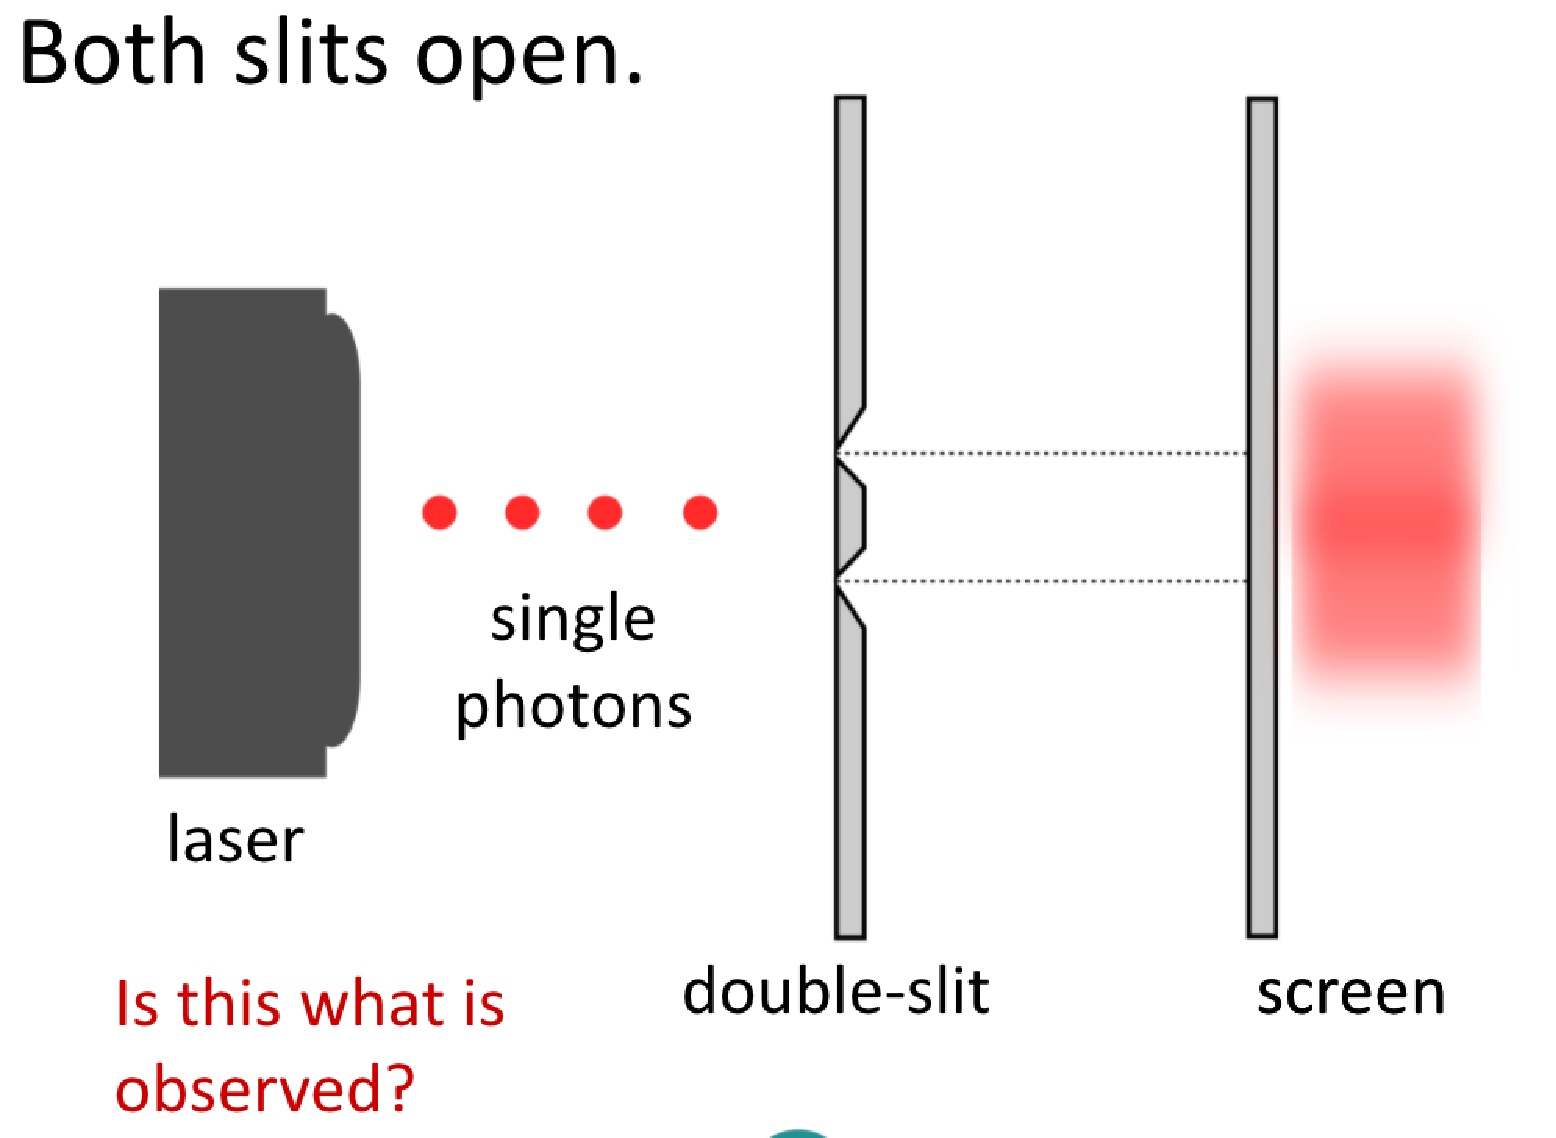
\includegraphics[width=0.8\textwidth]{lesson6/block_neither.pdf}
    
        \caption{When single photons are used and both slits are open, is this the pattern we observe?}
    \label{fig:two-slit-single-photon-wrong}
    
\end{figure}

In fact, we see the following: we start firing photons at the screen. Originally, there's not much pattern that we can discern, as on the left side of Fig.~\ref{fig:two-slit-single-photon-pattern}, but as time progresses, more and more photons hit the screen and we can clearly see these fringes being formed, as on the right side of the figure. These fringes are the same fringes we could see before with strong laser light. Let's pause and appreciate really what's going on. We saw these fringes on the right with a strong laser light, and it wasn't very surprising. Here, somehow each individual photon knows that they still need to follow the same pattern. Still they are drawn toward the bright fringes on the screen, and they avoid the dark fringes in between. This is because of interference of different possible paths. Even though we only have a single photon between the laser and the screen, still it obeys the same rules of interference as if we had a strong laser pulse.


% block neither reality
\begin{figure}[H]
   \centering
    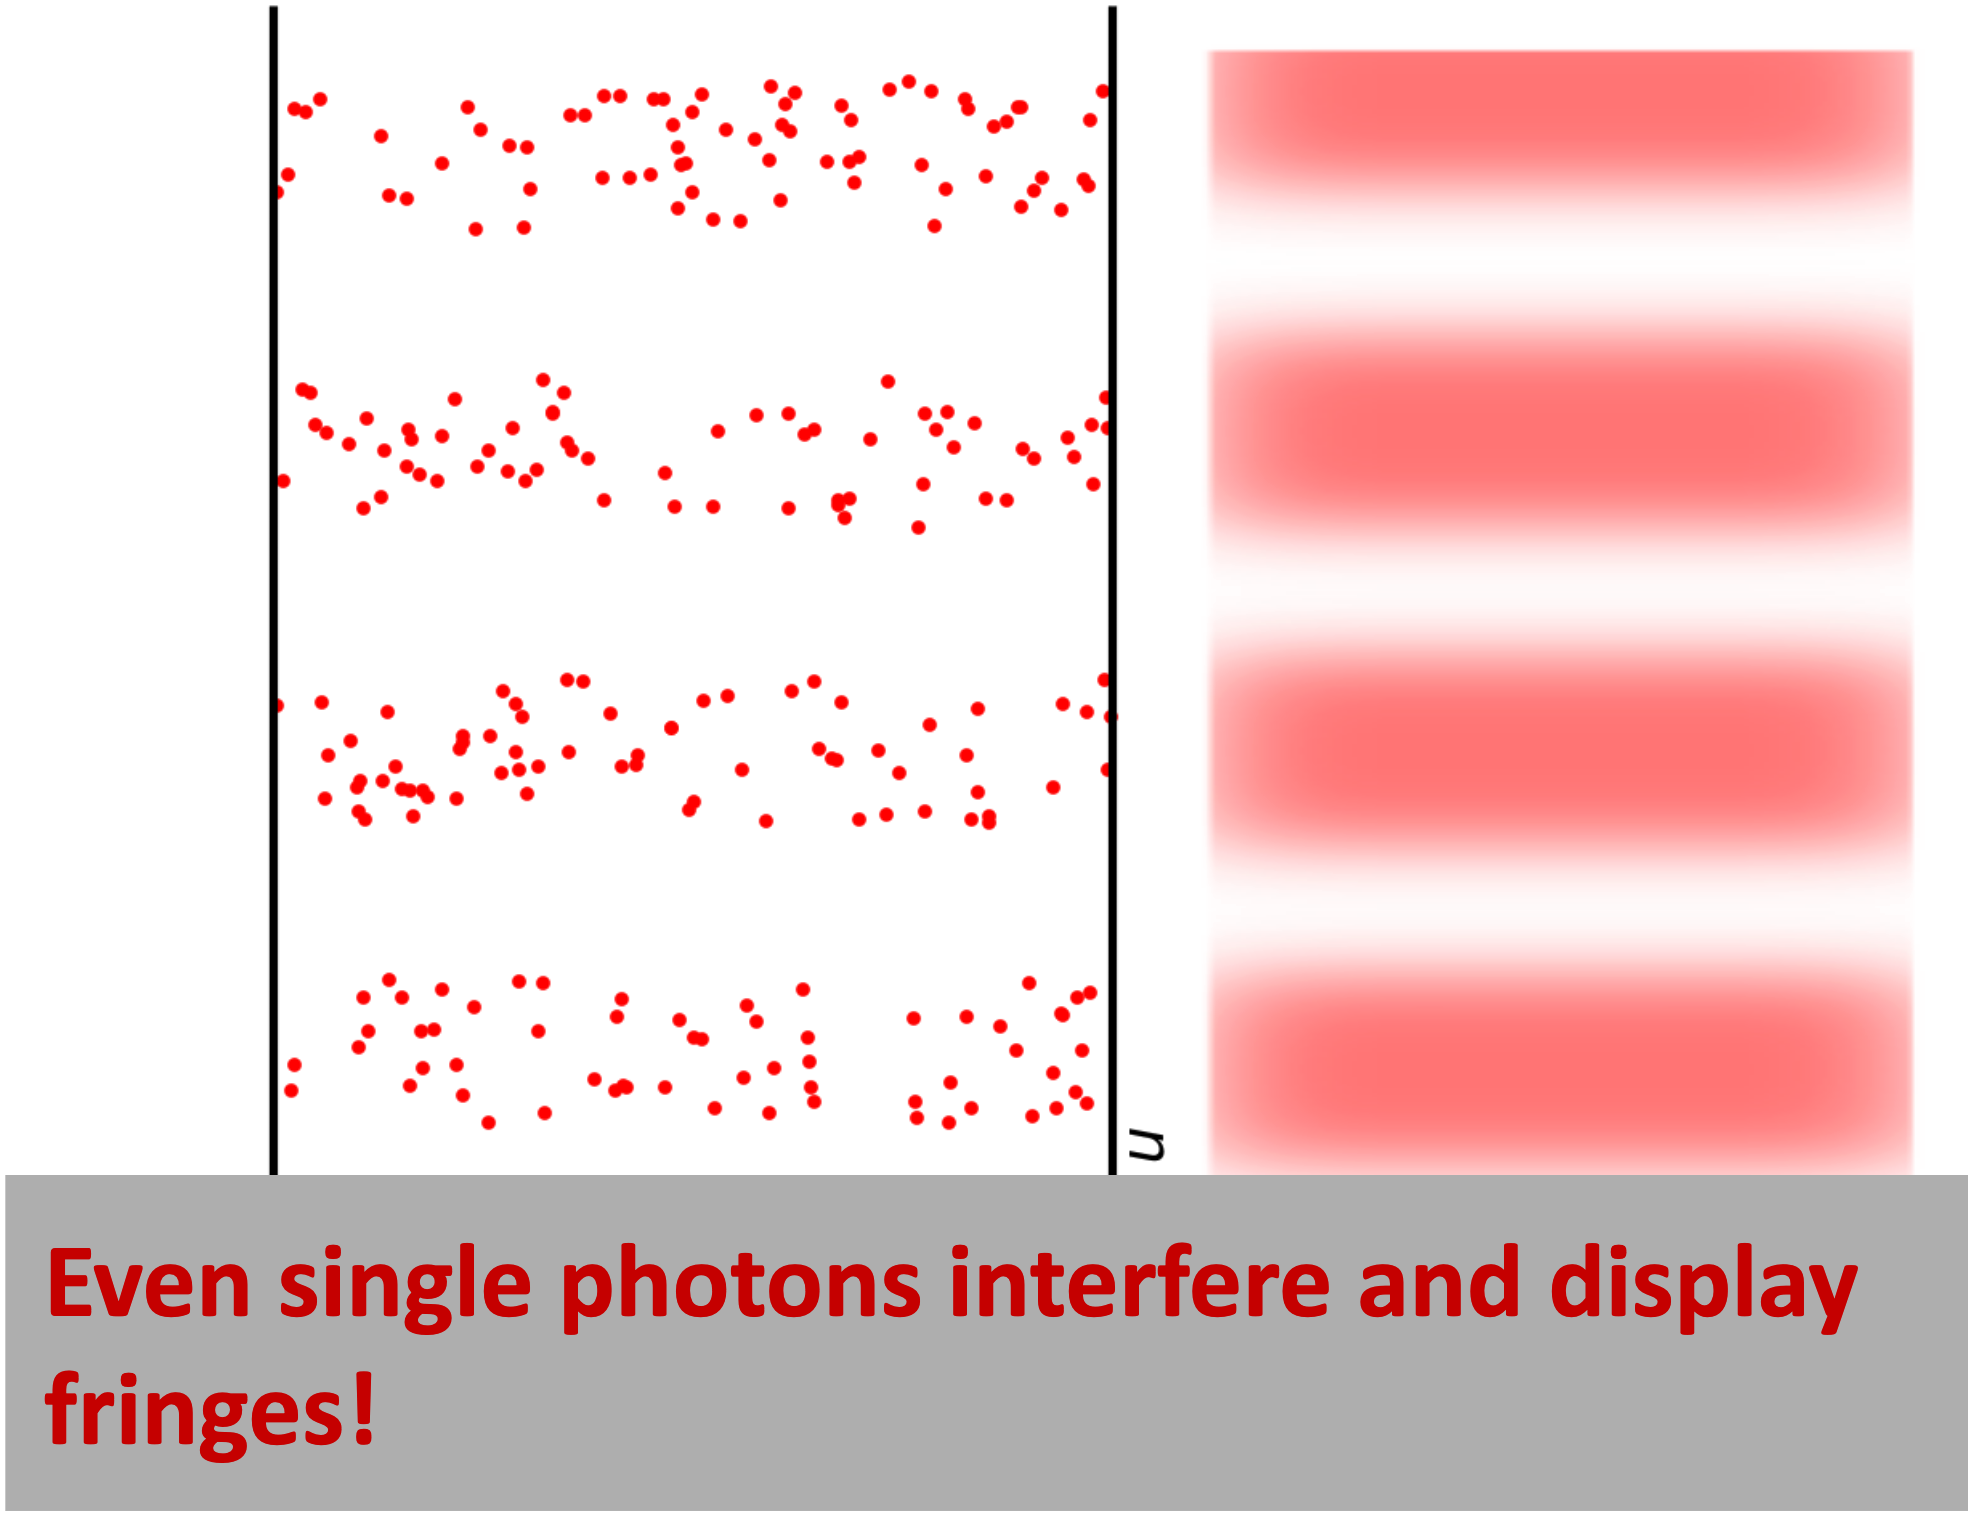
\includegraphics[width=0.8\textwidth]{lesson6/block_neither_reality.png}    
        \caption{In fact, when both slits are open, even single photons will create the same pattern after a large number of individual photons have accumulated.}
        \label{fig:two-slit-single-photon-pattern}

\end{figure}


\section{Interference with qubits}




We have seen how light interferes, how waves interfere, and even how single photons interfere. We can, in fact, see interference also with single qubits. Let's see how.

Consider that we have a Hadamard gate, and we apply it on the state of a qubit. We will consider two states: one is our state $\ket{0}$ which is given by the state vector (one zero), and the other is the state $\ket{1}$, which is given by its orthogonal friend (zero one), and the Hadamard gate $H$ is given by the transformation matrix,
\begin{equation}
\begin{aligned}
|0\rangle &=\left(\begin{array}{l}
1 \\
0
\end{array}\right) \quad|1\rangle=\left(\begin{array}{l}
0 \\
1
\end{array}\right) \quad H=\frac{1}{\sqrt{2}}\left(\begin{array}{cc}
1 & 1 \\
1 & -1
\end{array}\right)
\end{aligned}
\end{equation}

If we start in the state $\ket{0}$ and apply the Hadamard gate to it, we have seen that we create an equal superposition of state $\ket{0}$ and $\ket{1}$,
\begin{equation}
\begin{aligned}
|0\rangle & \longrightarrow H|0\rangle=\frac{1}{\sqrt{2}}(|0\rangle+|1\rangle)
\end{aligned}
\end{equation}
Now we can do the same thing again, we can apply another Hadamard gate to this superposition,
\begin{equation}
\begin{aligned}
H\left[\frac{1}{\sqrt{2}}(|0\rangle+|1\rangle)\right] &=\frac{1}{2}(|0\rangle+|1\rangle+|0\rangle-|1\rangle) \\
&=|0\rangle
\end{aligned}
\end{equation}
This can be seen by breaking the equation into its separate terms. From the first term, applying the Hadamard to the state $\ket{0}$ creates another superposition $\ket{0}+\ket{1}$. Applying Hadamard gate to the second term, the state $\ket{1}$ creates a superposition $\ket{0}-\ket{1}$. So after applications of two Hadamard gates, this is our state: the two $\ket{0}$ terms have the same sign and add up, or constructively interfere. The two $\ket{1}$ terms have opposite signs and cancel, or destructively interfere.
%You can see that these terms (0+1, 0-1), they both have a positive probability amplitude, plus a half, plus a half. Whereas the other two terms have opposite amplitudes, they've got plus a half, and negative a half. So the effect of that is that the probability amplitudes for ones cancel, whereas the probability amplitudes for the zeros, they constructively interfere, and we end up in a state zero which was our initial state, and this works also for state one if we use that as an initial state, but this time the cancellation of probability amplitudes happens for the zero terms, because they have plus one half minus one half, and the one terms, they constructively interfere because both of them have plus a half, plus a half probability amplitudes. So 
This may not surprise you too much. After all, applying Hadamard twice actually applies the identity, because the Hadamard gate is its own inverse.

So let's consider two different transformations. Let's call them BS1 and BS2,
\begin{equation}
B S 1=\frac{1}{\sqrt{2}}\left(\begin{array}{cc}
1 & 1 \\
1 & -1
\end{array}\right) \quad B S 2=\frac{1}{\sqrt{2}}\left(\begin{array}{cc}
-1 & 1 \\
1 & 1
\end{array}\right) \quad B S 2 \cdot B S 1 \neq I.
\end{equation}
You can see that BS1 is actually our previous Hadamard gate but let's just keep calling it BS1 for reasons that will become apparent a little bit later.  BS2 looks a little bit  like a Hadamard gate, but this time the minus is not located in the bottom right, but instead is in the top left. You can check for yourself that applying these gates in sequence is not the same thing as doing nothing. In particular, BS2 times BS1 is not equal to the identity.

But let's see what happens when we do apply them. Let's say our initial state is $\ket{1}$. We first apply the transformation BS1, then BS2, and what we get is the following
\begin{equation}
\begin{aligned}
B S 2 \cdot B S 1|1\rangle &=B S 2 \cdot \frac{1}{\sqrt{2}}\left(\begin{array}{cc}
1 & 1 \\
1 & -1
\end{array}\right)\left(\begin{array}{l}
0 \\
1
\end{array}\right) \\
&=B S 2 \cdot \frac{1}{\sqrt{2}}\left(\begin{array}{c}
1 \\
-1
\end{array}\right) \\
&=\frac{1}{2}\left(\begin{array}{cc}
-1 & 1 \\
1 & 1
\end{array}\right)\left(\begin{array}{c}
1 \\
-1
\end{array}\right) \\
&=\frac{1}{2}\left(\begin{array}{c}
-2 \\
0
\end{array}\right)=-|0\rangle=|0\rangle
\end{aligned}
\end{equation}
We apply the Hadamard gate to the vector (zero one), and after simple multiplication we get the superposition $\ket{0}-\ket{1}$. Then, we apply BS2, and what we get is in fact another translation. The probability amplitudes corresponding to state $\ket{0}$, they constructively interfere, whereas the probability amplitudes contributing towards state $\ket{1}$, they destructively interfere. Therefore the probability amplitude for state $\ket{1}$ becomes zero. The minus term that appears on the front is not important, it has no consequence because it's just a global phase, so we can just ignore it.
 
Now, let's consider an optical instrument called a \emph{Mach-Zehnder Interferometer}\index{Mach-Zehnder interferometer}\index{interferometer}, as shown in Fig.~\ref{fig:mach-zehnder}.
% Mach-Zehnder set-up
\begin{figure}[H]
   \centering
    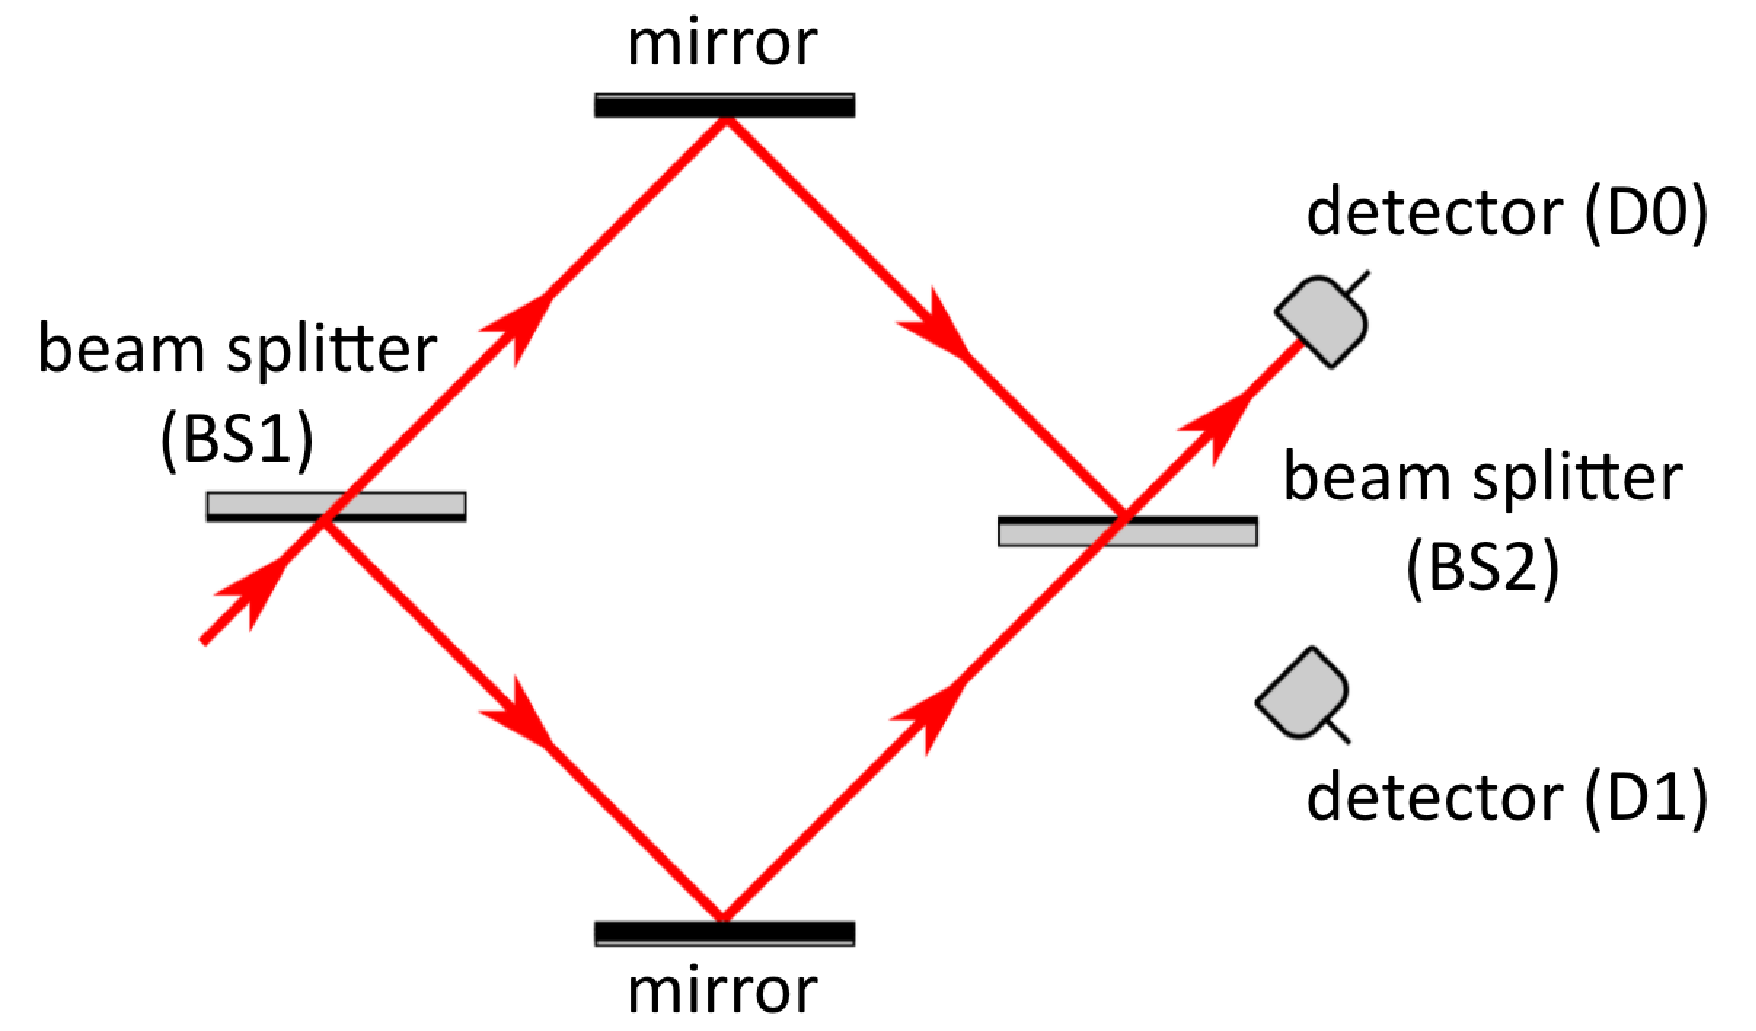
\includegraphics[width=0.8\textwidth]{lesson6/mach_zehnder.pdf}
    
        \caption{Mach-Zehnder interferometer.}
    \label{fig:mach-zehnder}
    
\end{figure}
It consists of two beam splitters which are BS1 and BS2, two mirrors, and two detectors.  The game that we like to play with this Mach-Zehnder Interferometer is this: we feed in some light into the first beam splitter, and then we ask the questions, "When will D0 click?  When will detector D1 click? What's the intensity measured at detector D0? What's the intensity measured at detected D1?" and so on. In this particular case, we assume that we only have light coming in from the bottom, and the mirrors and beam splitters are set in such a way that the path lengths are the same. The light can be reflected from the first beam splitter, bounce off the mirror, and enter the second beam splitter, or it can be transmitted through the first beam splitter, bounce off the top mirror, hit the second beam splitter interfere with the beam coming from the bottom branch, and it will be detected either at D0 and D1. If the path lengths are the same, then for this scenario, it will always be detected in the top detector D0.

That's what happens with strong, classical light. Now, let's consider what happens when only a single photon enters our Mach-Zehnder Interferometer, as in Fig.~\ref{fig:mach-zehnder-single-photon}. Again, the single photon can be reflected at the first one or transmitted. It bounces off the mirrors, which don't really do anything except alter the path of the photon.  The two paths then recombine at the second beam splitter, and we ask the question: is the photon detected at D0 or is it detected at D1?
% Single photon Mach-Zehnder case
\begin{figure}[H]
   \centering
    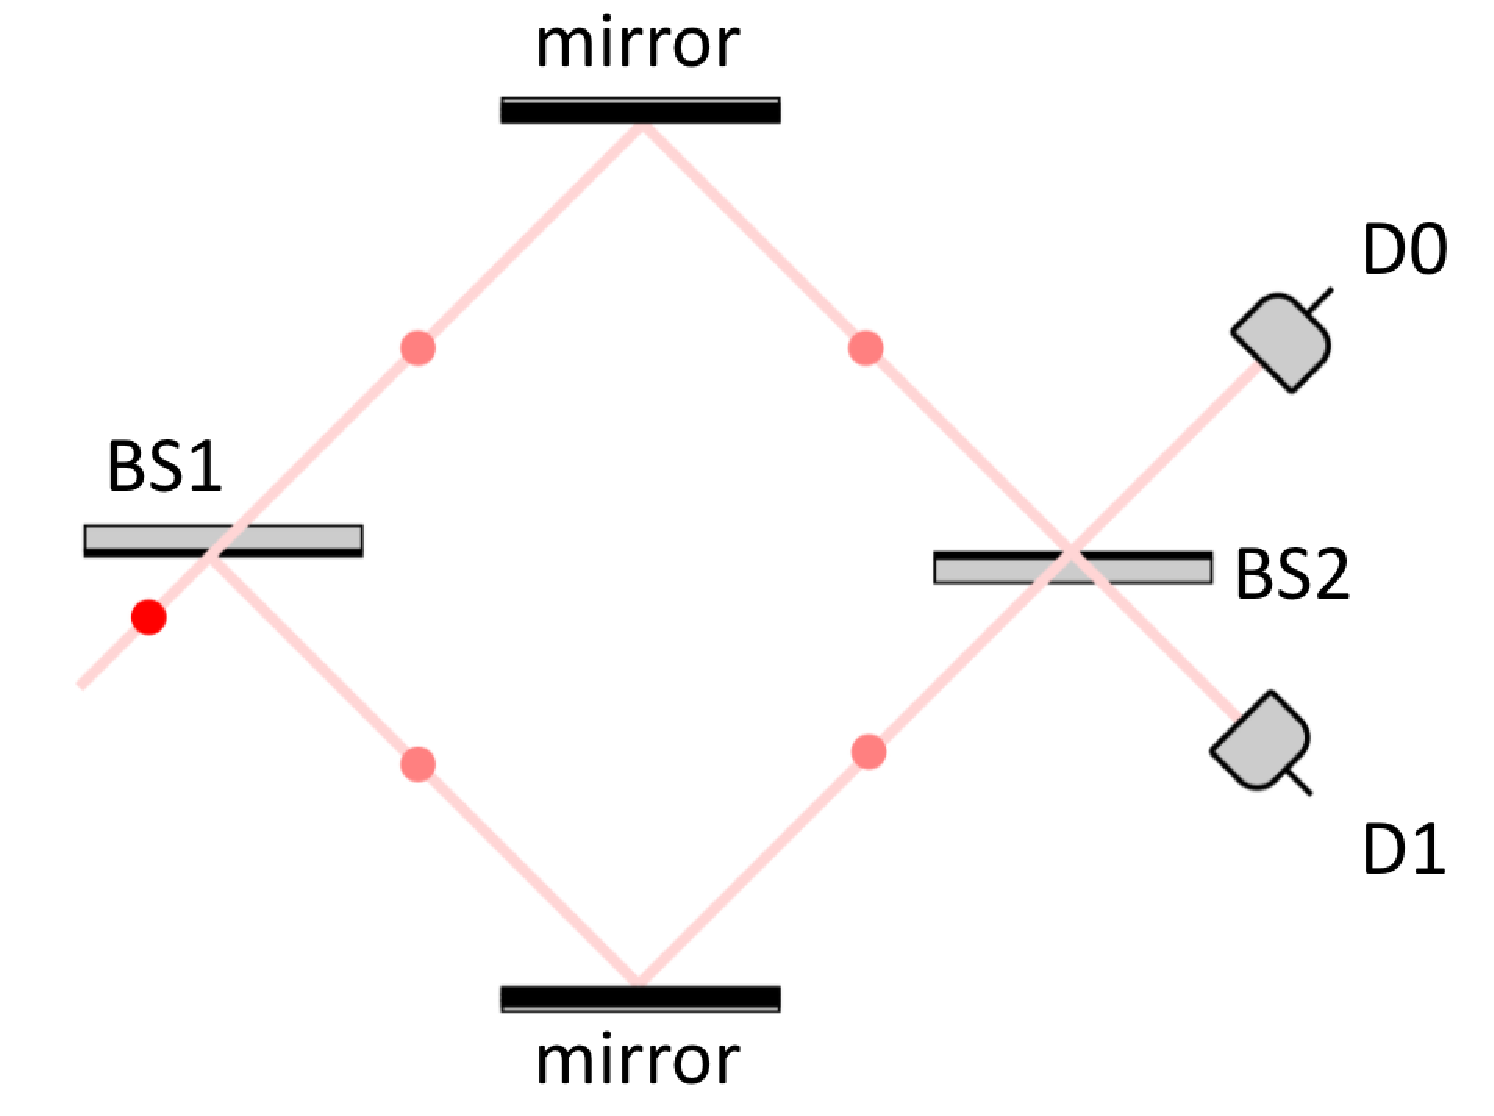
\includegraphics[width=0.8\textwidth]{lesson6/mach_zehnder_single_photon.pdf}
    
        \caption{Mach-Zehnder interferometer with a single photon.}
    \label{fig:mach-zehnder-single-photon}    
\end{figure}

In addition, the Mach-Zehnder Interferometer implements our qubit. How? Where is the qubit? Well, if the photon is found in the top half of the interferometer, we say that it's in the state $\ket{0}$, as in Fig.~\ref{fig:m-z-upper}. On the other hand if it's found in the bottom half, we say that it's in the state one, Fig.~\ref{fig:m-z-lower}. 
%So here the different paths encode different computational states of the qubit.

% 0 ket top
\begin{figure}[H]
   \centering
    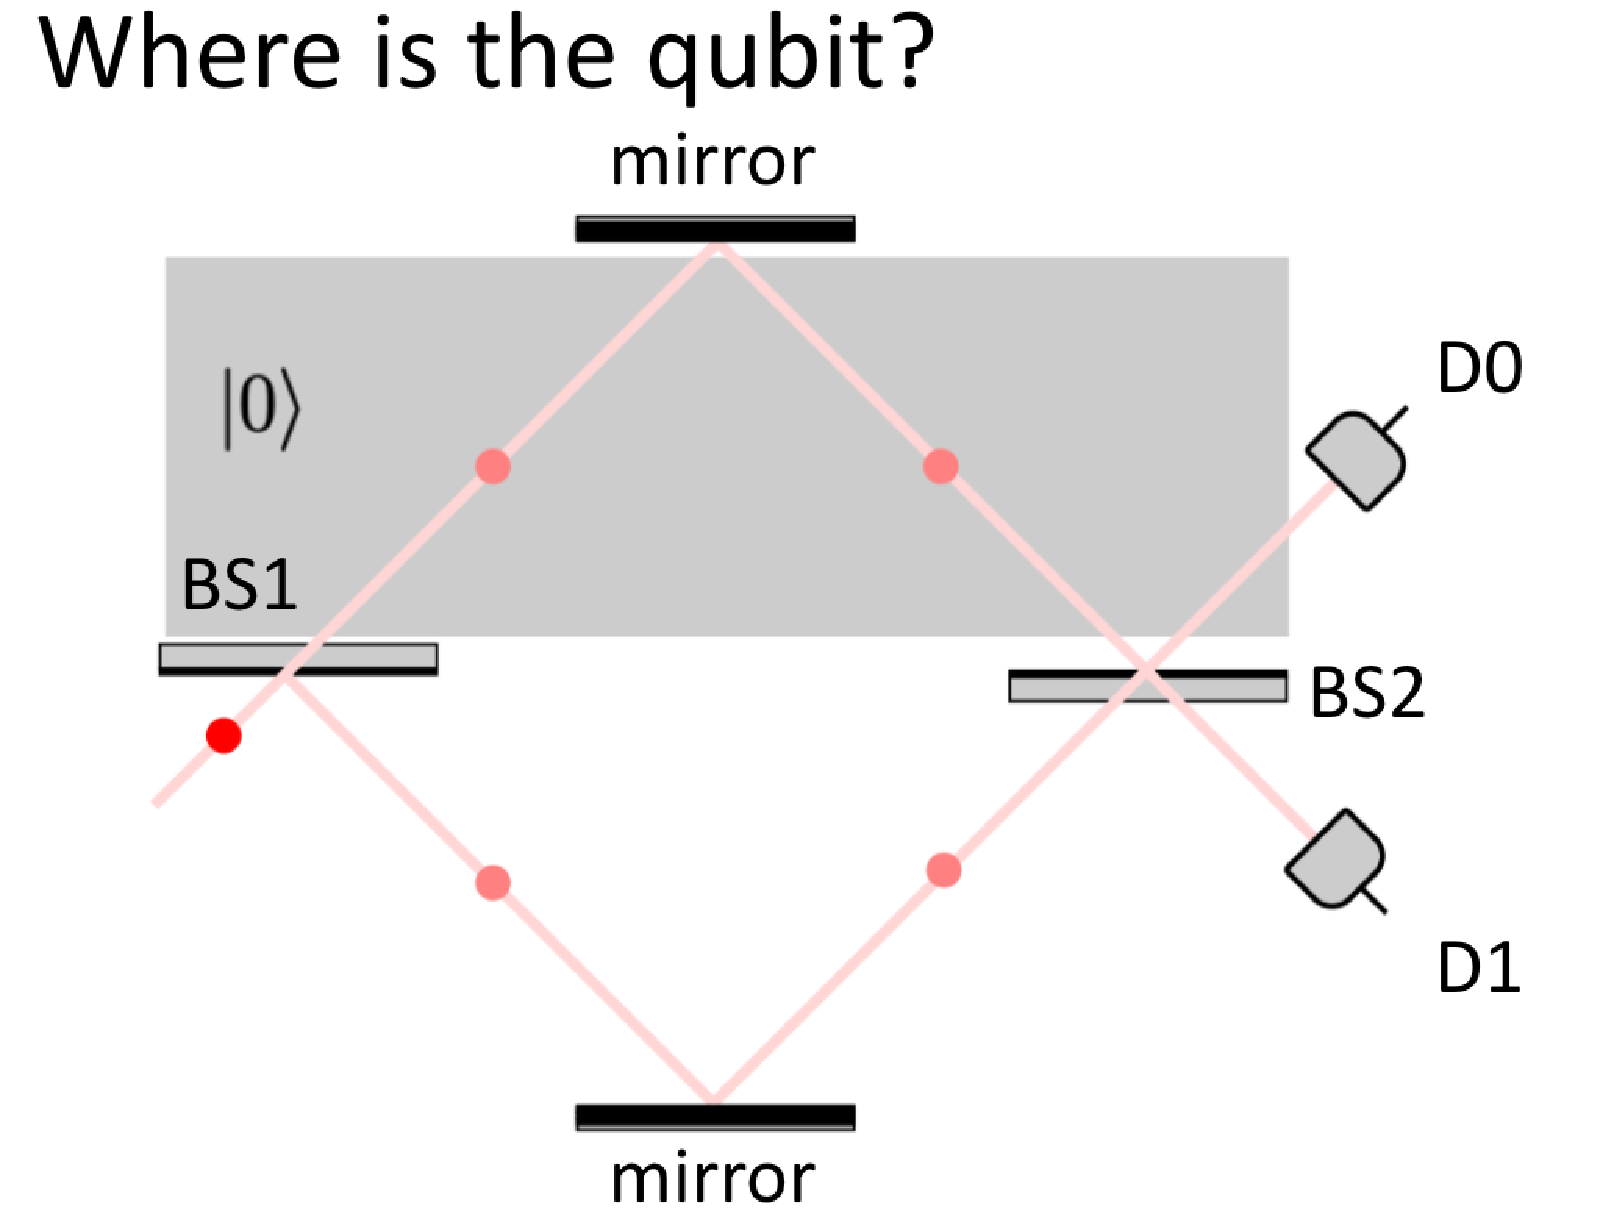
\includegraphics[width=0.8\textwidth]{lesson6/0_ket_botttom.pdf}
    
        \caption{$\ket{0}$ state is represented by a photon in the upper path.}
    \label{fig:m-z-upper}
    
\end{figure}

% 1 ket bottom
\begin{figure}[H]
   \centering
    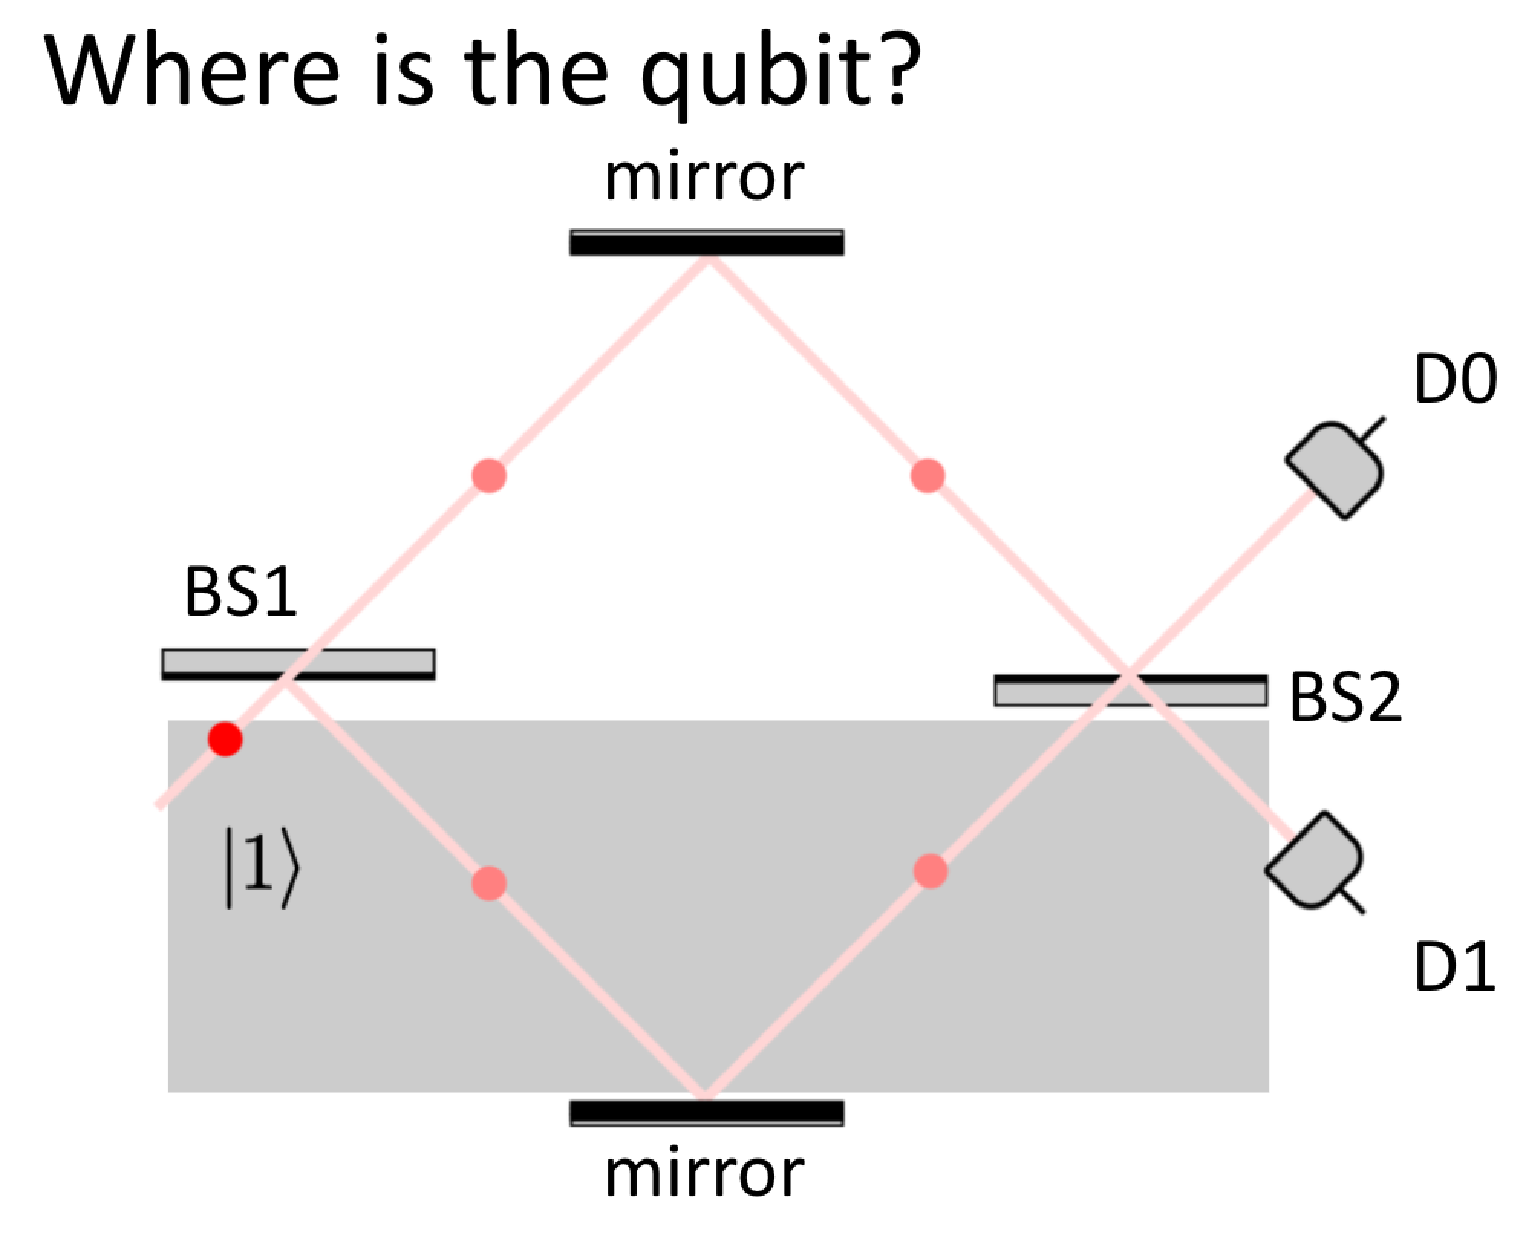
\includegraphics[width=0.8\textwidth]{lesson6/1_ket_bottom.pdf}
    
        \caption{$\ket{1}$ state is represented by a photon in the lower path.}
    \label{fig:m-z-lower}
    
\end{figure}

Let's consider our initial state to be $\ket{1}$, meaning it enters our Mach-Zehnder Interferometer from the bottom half.

Now you see why we have called those previous transformations BS1 and BS2. They correspond to the mathematical description of how these beam splitters affect the probability amplitudes of our qubit~\footnote{In fact, the quantum mechanical description of a beam splitter always has to involve writing down the state of both of the input ports to the beam splitter; here, we are being a little loose with the description. BS2 in this figure shows the correct accounting for photons coming from above and below the beam splitter, but for BS1 we have ignored the fact that we need to count the number of photons coming in from both above and below it, as well.  In future courses in this sequence, you will see a more rigorous treatment.}. We proved before that if we first act on our qubit with beam splitter one, and subsequently with beam splitter two, then we know that if the initial state is in the bottom half, then the output state will always be found in the top half, meaning D0 detector always clicks, as in Fig.~\ref{fig:m-z-d0}. The situation is very similar to the previous section. Here, there is only a single photon found in the Mach-Zehnder Interferometer. A photon is a single unit. There's always just one and it can't be divided, yet somehow it knows that it has to interfere with itself and always goes towards detector D0.

Now, let's do a simple test to better understand the behavior. Let's actually put some absorbing material and block the possibility of the photon going through the lower half of the Mach-Zehnder Interferometer, as in Fig.~\ref{fig:m-z-blocked}. What do we see? Well, the photon coming from below can get reflected at BS1. If it does get reflected, then it hits the block, gets absorbed and we don't get any clicks. However, if it gets transmitted at BS1, it bounces off the upper mirror and it is incident onto the second beam splitter, where again, it has an equal probability of being reflected or passing through the beam splitter. Therefore, it has a probability of being detected by both detector D0 and the detector D1. Effectively, by blocking this path of photon in the bottom of the Mach-Zehnder Interferometer, we have prevented interference from taking place at BS2. That is why we see both possibilities D0 and D1.

\if0
\begin{equation}
B S 2 \cdot B S 1|1\rangle=|0\rangle
\end{equation}
\fi

% D0 always clicks
\begin{figure}[H]
   \centering
    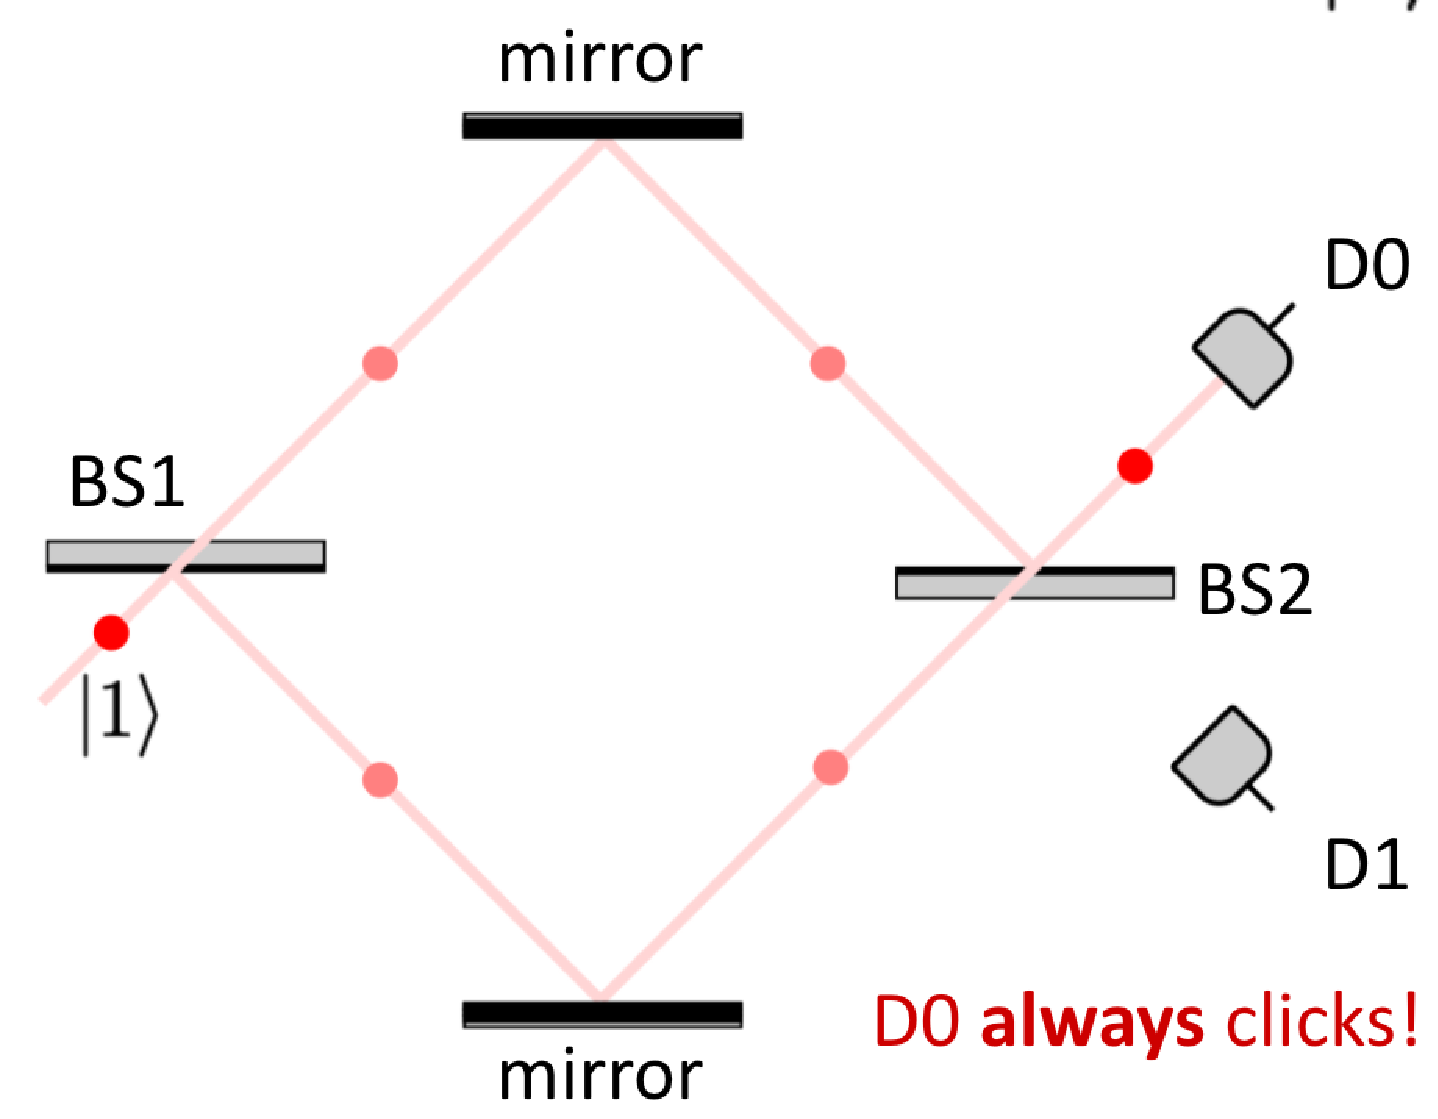
\includegraphics[width=0.8\textwidth]{lesson6/d0_always_clicks.pdf}
    
        \caption{$D0$ clicks with 100\% probability.}
    \label{fig:m-z-d0}
    
\end{figure}

% block bottom path
\begin{figure}[H]
   \centering
    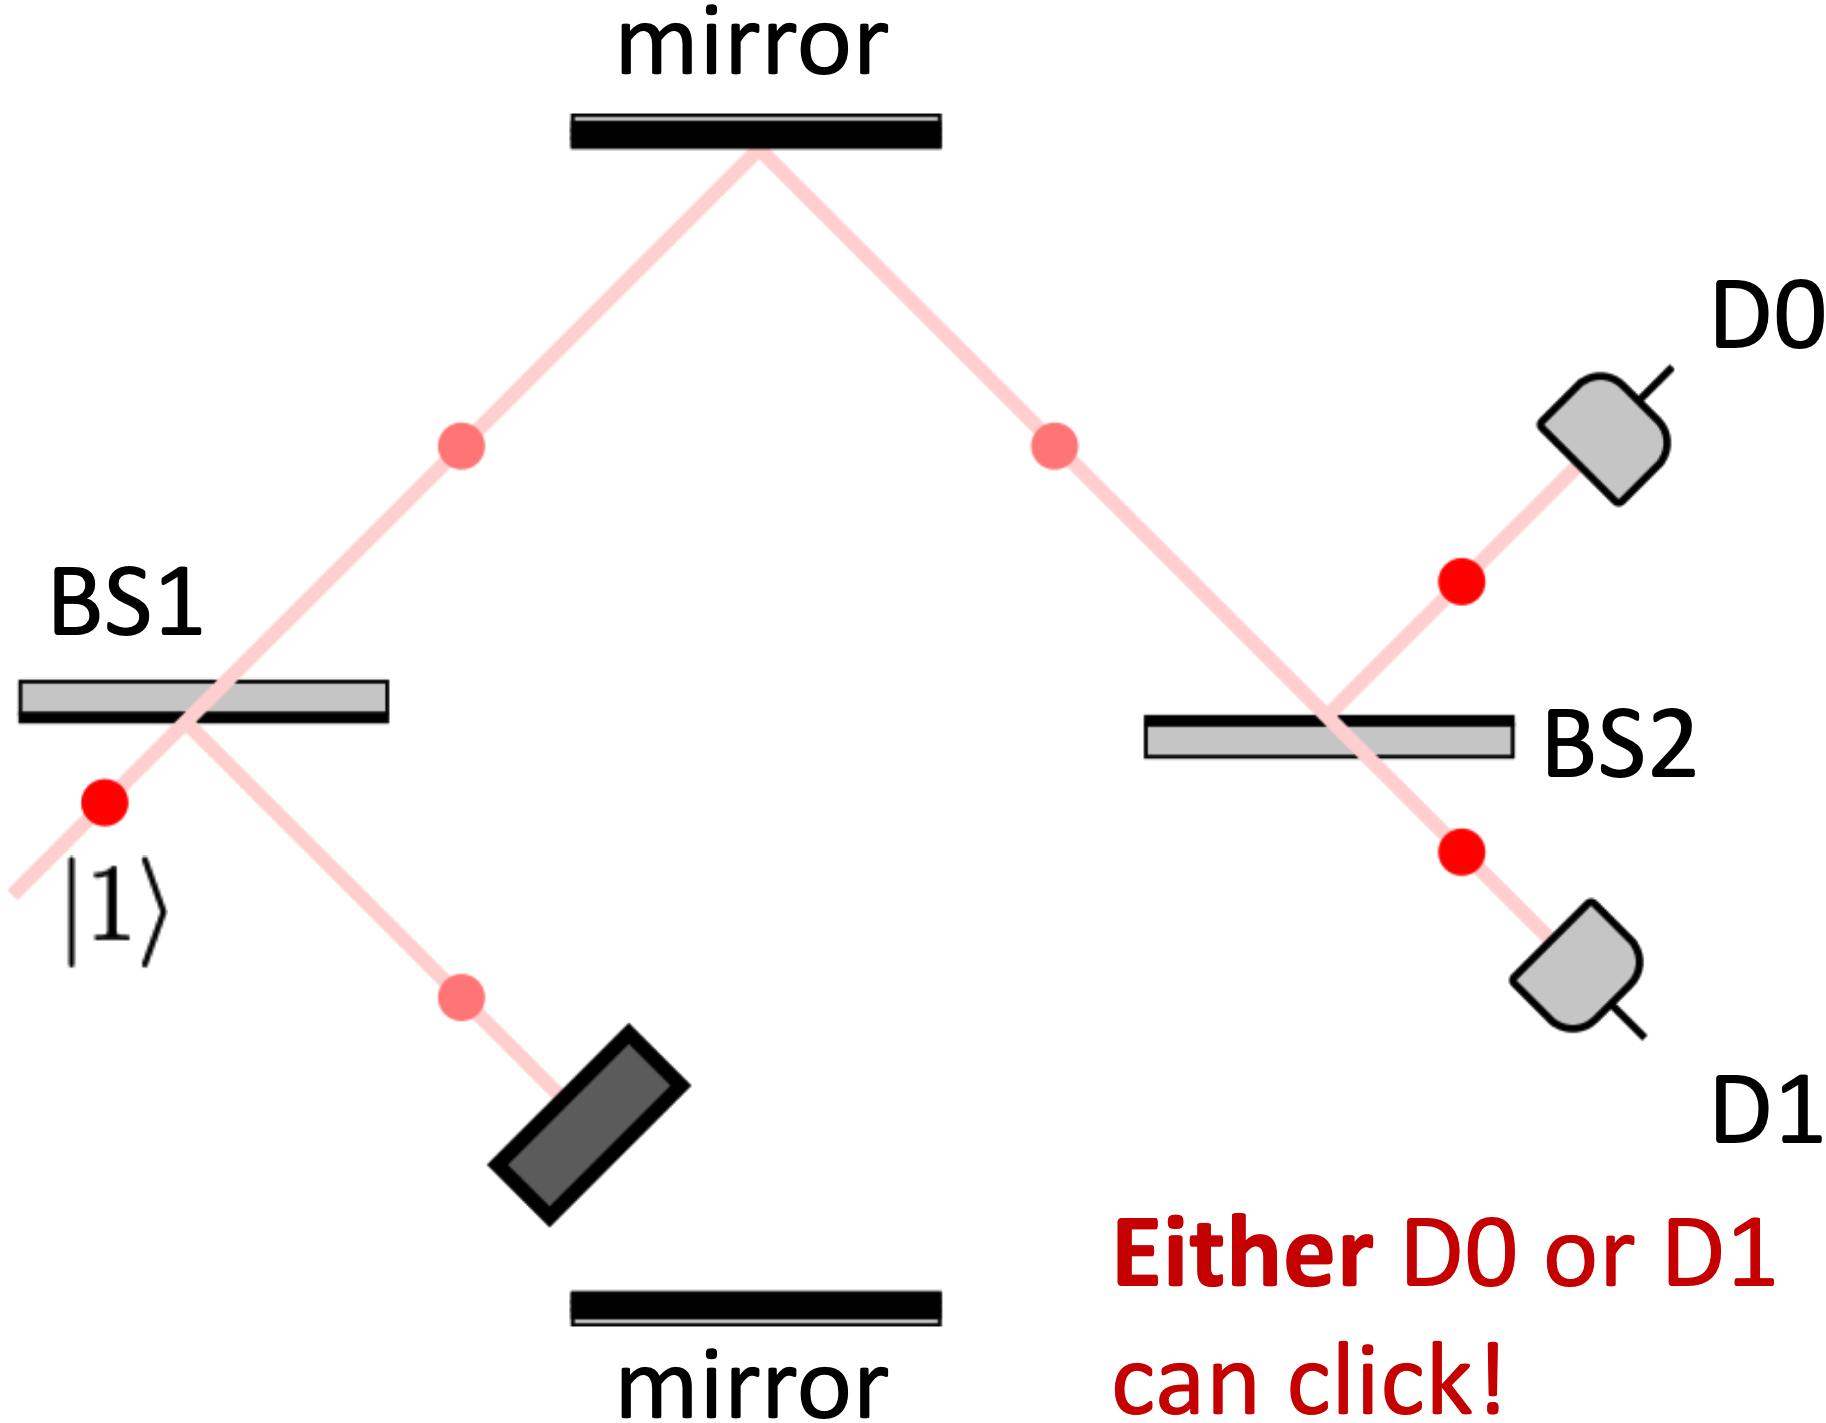
\includegraphics[width=0.8\textwidth]{lesson6/bottom_blocked.png}
    
        \caption{Lower path blocked. Because there is no photon coming from the lower path at BS2, no interference occurs, and any photon coming from above has a 50/50 chance of being directed to either detector.}
    \label{fig:m-z-blocked}
    
\end{figure}


\newpage
\begin{exercises}

\exer{Write some code to reproduce the static plot in Fig.~\ref{fig:decaying-superposition}.  Try to make your code represent the equations as nearly exactly as possible.  The plots and animations in our course were created using the Python package {\tt manim}, but your instructor may have different instructions for you.}

\exer{Write some code to reproduce the animated plot in Fig.~\ref{fig:propagating-waves}.  Try to make your code represent the equations as nearly exactly as possible.  The plots and animations in our course were created using the Python package {\tt manim}, but your instructor may have different instructions for you.}

\end{exercises}

